%%%%%%%%%%%%%%%%%%%%%%%%%%%%%%%%%%%%%%%%%%%%%%%%%%%%%%%%%%%%%%%%%%%%%%%%%%%%%%%%
%%  Sample document for preparing papers for  "Upravlenie bolshimi sistemami"
%%  charset=windows-1251
%%  The sample is based on the analogous sample of "Avtomatika i Telemekhanika".
%%%%%%%%%%%%%%%%%%%%%%%%%%%%%%%%%%%%%%%%%%%%%%%%%%%%%%%%%%%%%%%%%%%%%%%%%%%%%%%%

\documentclass[11pt]{ubs}
%%
%% для просмотра "as is" необходим набор русских шрифтов А. Лебедева
%% http://tex.imm.uran.ru/texserver/fonts/pscyr/pscyr4c/
%%

%_______________________________________________________________________________________________________
\usepackage{graphicx}
\usepackage{enumitem}
\usepackage{diagbox}
\usepackage{multirow}
\usepackage{empheq}
\usepackage{colortbl}
\usepackage{xcolor} % Для задания цветов
\DeclareMathOperator{\perprob}{P}
\DeclareMathOperator{\state}{\mathcal{S}}
\DeclareMathOperator{\action}{\mathcal{A}}

\definecolor{sfugrey}{RGB}{56,79,123}
%_______________________________________________________________________________________________________

\issue{XX}% Выпуск Сборника - проставляется в процессе верстки
\rubric{Программы и системы моделирования объектов, средств и систем управления}%  Рубрика Сборника - может быть скорректирована редактором
%
% Имеющиеся рубрики (последнюю информацию см. на сайте ubs.mtas.ru):
%
%    Системный анализ
%    Математическая теория управления
%    Анализ и синтез систем управления
%    Информационные технологии в управлении
%    Управление в социально-экономических системах
%    Управление в медико-биологических и экологических системах
%    Управление техническими системами и технологическими процессами
%    Управление подвижными объектами и навигация
%    Технические и программные средства управления
%    Надежность и диагностика средств и систем управления
%    Программы и системы моделирования объектов, средств и систем управления

% В соответствии с требованиями ВАК коды УДК и ББК обязательны. Проставляются автором. Могут быть скорректированы редактором
\udk{УДК ...} % Коды УДК можно найти на сайте https://classinform.ru/udk.html
\bbk{ББК ...} % Коды ББК можно найти на сайте https://classinform.ru/bbk.html

\title{Разработка адаптивной системы управления светофорными объектами с использованием марковских процессов принятия решений}% Название статьи
\engtitle{Article Title} % В соответствии с требованиями ВАК обязательно указывается название статьи на английском языке.

% Ссылка на грант и прочие благодарности. Оставьте команду \footnote и просто измените ее аргумент.
% Если ссылка не нужна, просто удалите следующую строку.
\thanks{\footnote{Работа поддержана Красноярским математическим центром, финансируемым Минобрнауки РФ (Соглашение 075-02-2024-1429).}}

% Список авторов должен вводиться в представленной форме. Авторы вводятся в алфавитном порядке.
% Сначала указывается Фамилия И.О., затем следует подстрочная ссылка (footnote) с полным именем,
% ученой степенью, должностью и контактной информацией (телефоном или e-mail-ом) автора,
% затем, с новой строки курсивом - организация, в которой работает автор.
% Если несколько подряд идущих авторов работают в одной организации, допускается перечислять их в одной строке,
% после которой идет строка с названием организации (см. пример ниже).
%
\authors{
%
\textbf{Тисленко~Т.И.}\footnote{Тисленко Тимофей Иванович, {(}timtisko@mail.ru{)}.},
\textbf{Семенова~Д.В.}\footnote{Семенова Дарья Владиславовна,\,д.ф.-м.н.,\,доцент {\makebox(20ex,1ex)[l]{{(}DVSemenova@sfu-kras.ru{).}
}
} }\\
\textit{{(}Сибирский федеральный университет, г.~Красноярск{)}}
%
}
%
\engauthors{% % В соответствии с требованиями ВАК обязательно указывается информация об авторах на английском языке.
\textbf{Alexander Ivanov}, Institute of Control Sciences of RAS,
Moscow, Cand.Sc., assistant professor (aaivanov@mail.ru). \\
\textbf{Boris Petrov}, Institute of Control Sciences of RAS, Moscow,
Doctor of Science, professor (Moscow, Profsoyuznaya st., 65,
(495)000-00-00). \\
\textbf{Vikor Sidorov}, Moscow Institute of Physics and Technology,
Moscow, student (viktor.sidorov@mipt.ru). }

\abstract{
В статье представлены результаты разработки программного комплекса MARLIN24, предназначенного для адаптивного управления светофорными \linebreak объектами. 
Структура комплекса включает  модуль адаптивного управления светофорными объектами, модуль симуляции движения транспорта и  модуль валидации. 
Математическая модель процесса управления светофорными \linebreak объектами --- управляемый марковский процесс с конечным числом действий и \linebreak  состояний. Задача поиска эффективного управления в целях  уменьшения суммарного времени нахождения  транспортных средств на детектируемых участках дорожной сети  сводится к задаче мультиагентного обучения с подкреплением (Multiagent Reinforcement Learning for Integrated Network, MARLIN).  Для поиска решения задачи MARLIN был построен алгоритм \linebreak $Q$-обучения.  
Структура программного комплекса также включает модуль  микросимуляции транспортных потоков  <<разумный водитель>> (Intelligent Driver Model, IDM).
Для имитации информации о реальной дорожной обстановке, поступающей в виде показаний оптического датчика,  в модуле валидации используются многомерные распределения, полученные с помощью применения копул Маршала-Олкина к маргинальным эмпирических распределениям для временных отметок  срабатывания оптического датчика.
Для построения маргинальных распределений использовались данные об интенсивности движения через детектируемые участки дорожной сети в период с 2019 по 2020 год.
}

% В соответствии с требованиями ВАК обязательно приводится расширенная аннотация на английском языке.
% Объем расширенной английской аннотации -- 150-200 слов.
% Английский текст проверяется редактором на предмет грамотности и соответствия русскому тексту и может быть изменен без согласования с авторами статьи.
\engabstract{%
% 150--200 words. Describes the standards of articles' formatting for "Large systems control" papers collection. Provides the examples for typical elements of an article. 150--200 words. Describes the standards of articles' formatting for "Large systems control" papers collection. Provides the examples for typical elements of an article. 150--200 words. Describes the standards of articles' formatting for "Large systems control" papers collection. Provides the examples for typical elements of an article. 150--200 words. Describes the standards of articles' formatting for "Large systems control" papers collection. Provides the examples for typical elements of an article.\newpage
}

% Обязательно указывается от трёх до шести ключевых слов
\keywords{
  имитационное моделирование транспортных потоков, модель IDM, модель MOBIL, копулы Маршалла-Олкина, машинное обучение с подкреплением}

% В соответствии с требованиями ВАК обязательно приводится перевод ключевых слов на английский язык.
\engkeywords{
  % large systems control, electronic scientific publication, article formatting template
}

\presented{...}% Член редколлегии, представляющий статью к публикации, заполняется редактором
\received{...}% Дата получения материала редакционной коллегией, заполняется  редактором
\published{...}% Дата опубликования статьи, заполняется редактором



\newtheorem{proposition1}{Утверждение}
\begin{document}

\maketitle

Одной из задач, решаемых в ходе реализации транспортной стратегии России на 2035 год \cite{transp_strat}, является увеличение пропускной способности и  скоростных параметров дорожной инфраструктуры до уровня лучших мировых достижений. При этом необходимо
учитывать  общесоциальные целевые ориентиры транспортной стратегии: подвижность населения, снижение аварийности, рисков и угроз безопасности по видам транспорта, снижение доли транспорта в загрязнении окружающей среды. Таким образом, актуальна проблема моделирования  транспортных потоков и оценки эффективности управления
светофорными объектами для наиболее нагруженных участков дорожной сети. %Эти инструменты  должны 

Системы, управляющие светофорными объектами, подразделяют на те, которые корректируют сигналы светофоров в реальном времени и реагируют на текущую дорожную обстановку --- АСУДД (адаптивные системы управления дорожным движением) и неадаптивные --- те, которые работают согласно фиксированному плану управления.
% Неадаптивные системы светофоров  переключают фазы светофоров через заранее заданное фиксированное время.
В таблице \ref{tab:adapt} представлены наиболее известные АСУДД, которые были разработаны в различные временные периоды и для различных условий движения.% (адаптивные системы управления дорожным движением).
\begin{table}[h!]
  \caption{Распространенные модели  АСУДД}
  \label{tab:adapt}
  \centering
  \scalebox{0.65}{
    \begin{tabular}{|c||c|c|c|c|c|c|}\hline
      \textbf{Критерий} & \textbf{UTCS-1}                       & \textbf{SCOOT}                          & \textbf{OPAC}                                                  & \parbox{0.2\textwidth}{\centering\rule{0em}{1.2em}\textbf{АСУДД} \\\textbf{<<Микро>>}\rule[-0.5em]{0em}{1.2em}} & \textbf{MARLIN}\\ \hline
      город             & Вашингтон                             & Лондон                                  & \parbox{0.2\textwidth}{\centering \rule{0em}{1.2em}Арлингтон,                                                                                    \\Тускон\rule[-0.5em]{0em}{1.2em}}  & Красноярск & Торонто\\ \hline
      \parbox{0.2\textwidth}{\centering\rule{0em}{1.2em}временной                                                                                                                                                                                            \\период} &1970е&1995&1983,1989 & 1993& 2010\\ \hline
      \parbox{0.2\textwidth}{\centering\rule{0em}{1.2em}длительность                                                                                                                                                                                         \\фаз\rule[-0.5em]{0em}{1.2em}} & \multicolumn{2}{c|}{фиксированная}  & \multicolumn{3}{c|}{переменная}  \\ \hline
      оптимизация       & офлайн                                & \multicolumn{4}{c|}{онлайн}                                                                                                                                                                \\ \hline
      предсказание      & нет                                   & \multicolumn{4}{c|}{есть}                                                                       \\ \hline
      устройство        & \multicolumn{2}{c|}{централизованная} & \multicolumn{3}{c|}{децентрализованная}                                                                                                                                                    \\ \hline
      \parbox{0.2\textwidth}{\centering\rule{0em}{1.2em}основные                                                                                                                                                                                             \\ограничения\rule[-0.5em]{0em}{1.2em}}   & \parbox{0.2\textwidth}{\centering\rule{0em}{1.2em}постоянный\\сбор данных} & \parbox{0.15\textwidth}{\centering \rule{0em}{1.2em}сенсоры \\далеко} & \parbox{0.2\textwidth}{\centering \rule{0em}{1.2em}только для\\  8 фаз}&  \parbox{0.2\textwidth}{\centering \rule{0em}{1.2em}находится \\в разработке} & \parbox{0.25\textwidth}{\centering <<ПРОКЛЯТИЕ\\РАЗМЕРНОСТИ>>} \\ \hline
      работы, авторы &&&&&\\\hline
    \end{tabular}
  }
\end{table}


Одна из ранних систем управления городским дорожным движением была UTCS-1 (Urban Traffic Control System)\cite{carini1977}. Система UTCS-1 использовала фиксированные сигнальные планы, которые менялись в зависимости от времени суток (утренний, дневной, вечерний планы). Для стабильной работы системы UTCS-1 необходимо  регулярно вручную корректировать сигнальные планы, что является существенным недостатком. На данный момент считается устаревшей, так как более современные системы UTCS-2, UTCS-3, SCOOT позволяют гибко управлять дорожным движением в реальном времени.

Система SCOOT (Split Cycle Offset Optimization Technique)\cite{chandler1985} анализирует данные о дорожной обстановке и корректирует светофорные сигналы, чтобы предотвратить образование заторов до их появления. Для работы данной системы требуется установка плотной сети индукционных петель, камер и других датчиков движения на расстоянии не менее  сорока метров и не более двухста метров до регулируемых перекрёстков. Централизованное управление SCOOT направлено на устранение <<эффекта волны>>. Однако продолжительность каждого сигнала светофора (Split) не указывает на изменение времени активной фазы в реальном времени.

Система OPAC (Optimized Policies for Adaptive Control)\cite{gartner1990} "--- это адаптивная система управления светофорами, схожая по назначению с системой SCOOT, но использующая другой подход для оптимизации транспортных потоков. OPAC, разработанная в США, предназначена для улучшения дорожной ситуации в реальном времени путем адаптации фаз светофоров в зависимости от условий трафика. В системе OPAC существует ограничение в восемь фаз для каждого светофора. Это ограничение связано с практическими соображениями, поскольку каждая фаза представляет собой отдельное направление движения или определённую комбинацию разрешённых манёвров на перекрёстке (например, движение прямо, поворот налево или направо). Эти ограничения заложены аппаратно, то есть на уровне контроллеров, и не могут быть изменены конечным пользователем.

Автоматизированная система управления дорожным движением (АСУДД) <<Микро>> \cite{asudd} "--- наиболее широко используемая в России система, успешно применяемая в следующих регионах:  Красноярский край, Иркутская область, Белгородская область, Воронежская область, Хабаровский край, Московская область. АСУДД <<Микро>> является децентрализованной системой и поддерживает до шести GPRS-серверов, которые позволяют подключить до 250 перекрёстков.  Детекторы АСУДД <<Микро>> работают на расстоянии до ста метров. Основным недостатком системы является тот факт, что реализация адаптивных алгоритмов  находится в стадии разработки.

В работах \cite{el-tantawy2013, tislenko2022a, tislenko2022b} для адаптивного управления светофорными объектами было предложено использовать  метод мультиагентного обучения с подкреплением.  
Данный подход получил название MARLIN (Multiagent Reinforcement Learning for Integrated Network) и  был успешно применен в современной АСУДД в Канаде. Целью обучения с подкреплением является сокращение времени проезда транспортных средств через выбранные участки дорожной сети. Управление светофорными объектами считается эффективным, если транспортные средства находятся на детектируемых участках менее двух циклов.
 Для работы требуется установка камер на расстоянии менее ста метров от стоп-линий. Агенты (светофоры) могут работать без информации о полной дорожной обстановке и управлять движением децентрализованно. Перечисленные особенности можно отнести к достоинствам подхода на основе MARLIN. Существенным ограничением является рост вычислительной сложности при увеличении обзора агента, известный как <<проклятие размерности>>.

% Как альтернатива к применяемым на практике АСУДД, в работе  предложен метод адаптивного управления, использующий  мультиагентное обучение с подкреплением (Multiagent Reinforcement Learning for Integrated Network, MARLIN)\cite{MARL}, основанные на марковских процессах принятия решений, которые могут и не оперировать интенсивностью проезда через поперечное сечение дороги.



% Во {введении }  дается краткий обзор наиболее известных систем адаптивного управления светофорными объектами. Приводятся особенности реализации.

Фокус наших исследований сосредоточен на   разработке программных и математических инструментов для адаптивного управления сетью светофорных объектов участков дорожной сети города Красноярска. 
В настоящей работе представлен новый программный комплекс MARLIN24, реализующий часть методов новейших АСУДД. Оценка эффективности применяемого управления и валидация полученных результатов осуществляется с помощью симуляционных экспериментов на основе статистических данных с оптических детекторов за  2018 и 2019 года. 

Структура статьи следующая. В {параграфах  \ref{par:MARL_description}} и \ref{par:MARL_many_description}
проблема управления 
светофорными объектами сводится к задаче мультиагентного обучения с подкреплением для одного и нескольких агентов соответственно. 
\textcolor{red}{дописать текст из файлика в оверлифе}

\section{Общее описание программного комплекса MARLIN24}

Структура программного комплекса MARLIN24 приведена на рисунке~\ref{fig:structure_MARLIN24} и состоит из четырех модулей:  симуляции,  валидации,  адаптивного управления светофорными объектами, визуализации. 
% \red{опционально отключаемы}
% \red{посмотреть статьи с приложениями/ перенести в приложения }
\begin{figure}[tbph]
  \centering
  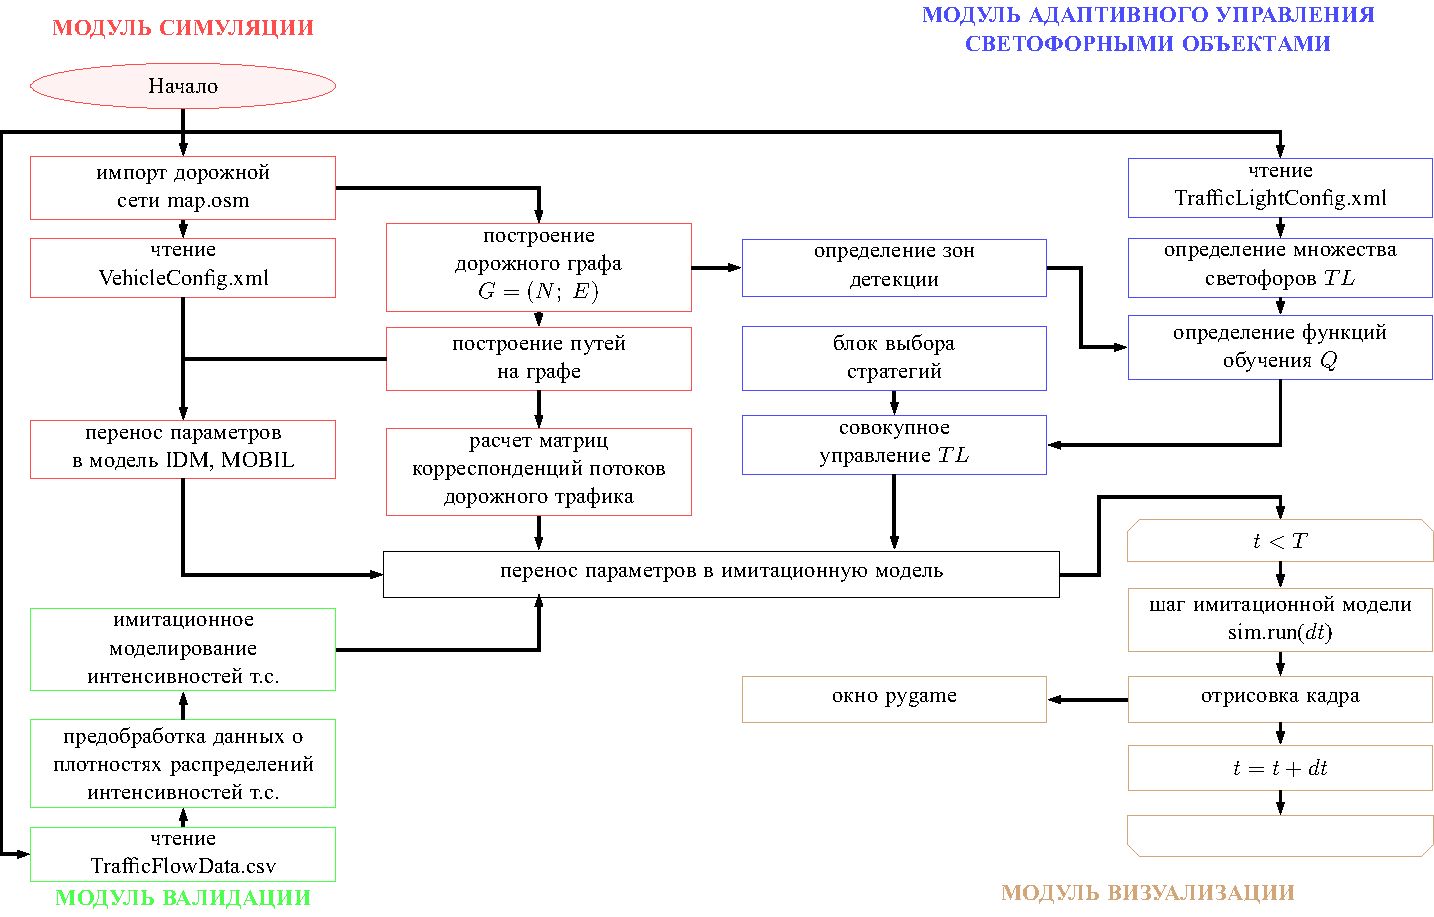
\includegraphics[width=0.99\textwidth]{structure.pdf}
  \caption{Структура программного комплекса MARLIN24}\label{fig:structure_MARLIN24}
\end{figure}


Модуль симуляции предназначен для оценки эффективности выбранного управления. 
Он реализует микросимуляционные модели движения, предназначенные для описания перемещения транспортных средств по дорожной сети. 
Часть программного кода, отвечающая за валидацию,  позволяет    моделировать интенсивности движения транспортных потоков. 
Включение модулей является опциональным, так графический интерфейс в модуле визуализации  позволяет производить визуальную оценку применяемого управления. Данный модуль отображает транспортные средства, дорожную сеть, дополнительную информацию о содержании названий дорог, их координатах. Также в модуле реализована функция ускорения и замедления модельного времени, выделения маршрутов, масштабирования и перемещения зоны обзора.

\section{������ ���������}
\label{par:MARLIN24_sim}
������ ��������� ������������ ��� ������ ������������� ���������� ���������� ������������ ���������.
� ������ ����������� ��� ������������������ ������ ��������, ��������������� ��� �������� ����������� ������������ ������� �� �������� ����. 
������ ������ IDM (Intelligent Driver Model) ��������� �������� ������������ ������� �� ������������ ������ ������ \cite{IDM}. ������ ������ --- MOBIL  (Microscopic Optimally Balanced Intersection Lanes) ��������� ������������ �� ������������� ������ \cite{MOBIL}.
� �������� ��������� �������� ������������ ������� 
 ����������� ���������� ������ � �������  �����������  ��������, � ����� ������������� ������������  ��������� ���������� �������� � ������ ����������.

\subsection{������ �������� ������������ �������}
\label{subpar: IDM_math}
��� �������� �������� ������������ ������� ������������ ������ IDM.
%� ������ �������� ������������ ������� ���������� 
������ ������ ��������� ��������� ��������� ���������: ����������� ���������� ���������, ������������ ����������� �������� � ����������� ���������� ������������ �������.
%������ ���������  ����� ��������� ������������ ������� ��� �������� ����������� �������� �������� ����. 
� ����� � ���� ������������ ������������ �������������� ������  ����������������� �������� IDM, ������� ��������� ��������� �������� � ������ ��������� ����������.
� ������� \ref{table:transp_definitions} ������������ �������� ���������� ��� ������ IDM, ������������ ����� � ������.
\begin{table}[tbph]
    \caption{�������� ����������� ��� ������ IDM }\label{table:transp_definitions}
    \centering
    \scalebox{0.68}{
    \begin{tabular}{|c|p{0.7\textwidth}|}
        \hline
        ������                        & ��������                                 \\
        \hline
        \rule{0em}{1.3em}${i} $       & ����� ������������� ��������              \\\hline
        %\rule{0em}{1.3em}$j$ & ��������� �� $i$ ���������� �� ������� ��� ������������ ������ ��������  \\\hline
        \rule{0em}{1.3em}${s}_{0,i} $ & ����������� ���������� ��������� ��� �.�. $i$ \\\hline
        \rule{0em}{1.3em}$v_{0,i}$    & ������������ ����������� �������� $i$    \\\hline
        \rule{0em}{1.3em}$\delta $    & ���������� <<���������>> ���������       \\\hline
        \rule{0em}{1.3em}$T_i$        & ����� ������� $i$-�� ��������            \\\hline
        \rule{0em}{1.3em}${a}_i $     & ��������� $i$               \\\hline
        \rule{0em}{1.3em}$ b_i$       & ����������� ���������� $i$                \\\hline
        \rule{0em}{1.3em}$s^\ast$     & �������� ���������� ����� $i$ � $i-1$   \\\hline
        % \rule{0em}{1.3em}$\widetilde{a}_{i}$ &  ��������� ������������� �������� $i$ ����� ��������� �������� ����������\\\hline 
    \end{tabular}}
\end{table}


� ������ IDM ��� ������������  �������� ��������������� ��� �������������� ��������,  ����������  ���������������� � ����������.
������ IDM ��������� � ������ ������� �������� �� �������,  ��� �������� �� �������������� ����� ������������, ��� ������ �������� ���������� �������� ������ ���������� � ����������� �� ���������� �� ������� ������� ����������, ��� �����\-��� � ����������� �����\-���.
�� ������� \ref{fig:IDM_illustration} ������������ �������� ������������ � �������������� �������� ����������, �������������� � $i$-��  �������, � $(i-1)$-�� ����������, ������������ ����� ���.
\begin{figure}[tbph]
    \centering
    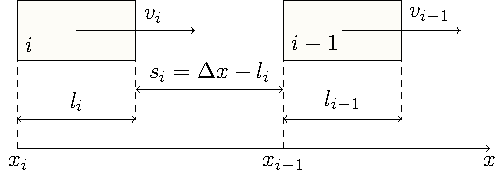
\includegraphics[width = 0.65\textwidth]{sim_descr.pdf}
    \caption{����������� ������ IDM}\label{fig:IDM_illustration}
\end{figure}



������� ���������, ����������� ������� ��������  $i$-�� ����������  � ���������� �� $(i-1)$-�� ���������� � ������ IDM � ������������ ������������ ����� ���:
\begin{equation} \label{eq:IDM_sys}
    \left\{
    \begin{array}{l}
        \displaystyle   \frac{dv_i}{dt}=
        \underbrace{a_i\Biggl( 1-\left(\frac{v_i}{v_{0,i}}\right)^\delta\Biggr)}_{\displaystyle a_{\mathrm{free\;road}}}-
        \underbrace{a_i\Biggl( \frac{s^*\left(v_i\Delta v_i\right)}{s_i}\Biggr)^2}_{\displaystyle a_{\mathrm{deceleration}}}, \\
        \displaystyle
        s^*\left(v_i, \Delta v_i\right)=s_{0,i}+v_iT_i+\frac{v_i\Delta v_i}{2\sqrt{a_ib_i}}.
    \end{array}\right.
\end{equation}



��� ������������ ������������� ��� ���������� �������� �����\-��� � ���������  ����� ������������ ���������, ����������� �� ���������� ������ <<����������>> \cite{SHOOT}:
\[
    \left\{
    \begin{array}{l}
        \displaystyle\frac{dv}{dt}(t) =  a_{\mathrm{free\;road}}(t)+a_{\mathrm{deceleration}}(t),        \\
        \displaystyle v(t+\Delta t)    =  v(t) + \frac{dv}{dt}(t)\Delta t,                               \\
        \displaystyle x(t+\Delta t)    =  x(t)+v(t)\Delta t+ \frac{1}{2}  \frac{dv}{dt}(t) (\Delta t)^2, \\
        \displaystyle s(t+\Delta t)    =  x_i(t+\Delta t)- x(t+\Delta t)- {l}_i.
    \end{array}
    \right.
\]
���  ��������� $dt$ ���������� ��� ��� �� ������� ��� ��������� ������� ������� (\ref{eq:IDM_sys}).

������������ ������������ ������ IDM �������� �� ������������ ������ � ������������� ��������.
����� �� �������� ��������� �� ������������ � ������������� �������� ����� �������� �������� ����������, ����������� ������������ ������������ �������.
� ������ ������������ ������ MOBIL.

� ������ ������ MOBIL ����� ���� � ���, ��� �������� ��������� ������� � ������������ � ��������� �������� �������� �� ����������� ������������ � ������������.
���������� ��������� ������ ��������, �������� � ������ ������ �������� �� ����� ������, ��� �������� �� {�������~\ref{fig:MOBIL},} �������, ��� �������, �� ���� ��������� ������������ ������� �� ������� ������ �������� � �������������� �� ������� ������ ��������.

\begin{figure}[tbph]
    \centering
    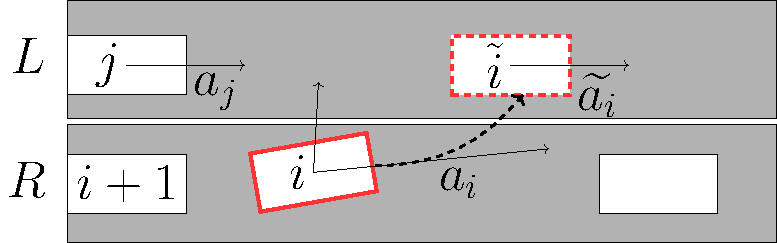
\includegraphics[width = 0.5\textwidth]{mobil.pdf}
    \caption{������ ����� ������ MOBIL}\label{fig:MOBIL}
\end{figure}

������ ��� ������������ ����, ���� ����� ������� ����������  ������������  � ������ ������ $R$ �� ����� ������ $L$ ����� ������������  ���������  �������� ������ IDM � ��������� �������� ������������ ������� ���� �� ����� ��������� $\delta$:
{
\abovedisplayskip=-0.0em
\belowdisplayskip=0em
$$
    R\to L: \quad \left(\widetilde{a_i}-a_i \right) + m\left((\widetilde{a}_{i+1}-a_{i+1})  + (\widetilde{a_j}-a_j)  \right) \geqslant \delta,
$$ }
\noindent
���  $m \in \left[ -\infty;\frac{1}{2}\right]\cup  \left[1; +\infty\right]$ ---  ������� ���������� ����������� ����������, ������ $\;\widetilde{}$ ���������� ���������� ��������������.
��������  ������������� \cite{MOBIL} ������������ ���������� $m$:
{
\begin{description}[itemsep=-3pt, topsep=0pt]
    \item[ {$\mathit{m > 1, }$                                } \textit{�������������� ���������}:] �� ���������������, \;\;\;\; ���� ��� �������  ����� �������� ��������;
    \item[ {$\mathit{0 \leqslant m \leqslant 0.5, }$  } \textit{������������ ���������}:  ] �������� ������ \;\;\;\; ������������ ������� ����� �����������;
    \item[ {$\mathit{m<0, }$                                  } \textit{������������� ���������}: ] ��������  ������������� \;\;  ��������  ���������� ��������� ���������. %\red{����� ��������� ��������� ��� ��� ��������� �� ������� ����}. 
\end{description}
}
����� ������� ���������, ��� ��� ������������ $i$ �� �������� ������ ������������ �������� $j$ � ��������� �� ��� ������ ��������� � ������������� ���������� ������, ��� $b_{\mathrm{safe}}.$ ��������� � ������ IDM ��������, �, �������������, � ��������� ������� ��������   (\ref{eq:IDM_sys}) � ���������� ��������������� �� ����������� ������������� �������� � ������������, �� ������� ����� ���������� ����� ��������:
$
    \widetilde{a_j} \geqslant -b.
$
\subsection{�������� ������ ������}
������ ��������� ������� ��  ���� �������� ���������������� ����  {VehicleConfig.xml}, � ������� ���������� ����� ��������� ��� ����������� ����������� ��������, ����������� ���������� (�������� ������),  ���������� �����.
�������������, � ������ ���������  ���������  ���������� � �������� ���� � ���� ����������� {map.osm},  ���������������� ����������� osmnx \cite{osmnx}.
��� ����������  ���������  ������������ �������  � �������� ����  ������������ ����������  networkx \cite{networkx}.

������ ��� �� ������� $t$ � ������ ��������� ����� ���� ��������� � ������ ������������ � �������������� ���������� pygame.
������ ������������ ������������ �������� ����, ������������ �������� � ���������� ����������, � ����� ��������� �������� ��������� �����.
% ������������� ����������� ������� � ������ ��������� ����������� �������� ������� ������� � ������������ ������� ���������� �����������.


% ��������� ���������� ��������� ���������� �������� ������ ���������� �������,  �� ��� ��������� ������������� ������ ������������   ������������� ���������� ��������� ���������� ��������� ��� ������ ������  threading\cite{python-threading}.
% ��� ���������� ��������, ���� �������� ������������� ���������� ����� osmid. ������ ������� ������������ ���� (�����������, ������������ ���������� �������) ��� ����� ������������� ��������� ������������� ������.  ������ ����� ������������� ��������� ������� ������ ��� ������������.
% � ������ �������� ���������� � ����������� ��� ��������, �� �����������, ����� ������, ���������� �����, �������� �����, � ����� ������ ���������� �� ����. \ref{table:road_params_OSM}.

% \begin{table}[h!]
%     \caption{������������� ��������� ����� �� OSM}\label{table:road_params_OSM}
%     \scalebox{0.72}{
%         \begin{tabular}{|l||l|l|}\hline
%             \rule{0em}{1.5em}\textbf{��������} & \textbf{����������� ��������}                                                                       & \textbf{��������} \hfill                                                                                                                             \\\hline
%             lanes                              & int                                                                                                 & ����� �����.                                                                                                                                         \\\hline
%             highway                            & \begin{tabular}[c]{@{}l@{}}residential\\ primary\\ secondary\\ terliary\\ unclassified\end{tabular} & \begin{tabular}[c]{@{}l@{}} ������ ����� ���,\\ ������������,\\ ����������,\\ �������� ��������,\\ ���������� �������������� ���� �����\end{tabular} \\\hline
%             lanes                              & str                                                                                                 & �������� �����                                                                                                                                       \\\hline
%             oneway                             & bool                                                                                                & ������, ������� �������� ������ ����� ���                                                                                                            \\\hline
%             reversed                           & bool                                                                                                & \begin{tabular}[c]{@{}l@{}}����������� �������� ����� \end{tabular}                                                                                  \\\hline
%             length                             & float                                                                                               & ������ ������                                                                                                                                        \\\hline
%         \end{tabular}}
% \end{table}


\section{������ ���������}
\label{par:MARLIN24_val}
% \textcolor{red}{���� ���� ��� ��� ��������}

� ������ ���������  �������� ������ ������������� ������������� ������������� �������� ������������� ������. � ������ ������ ��� �������������� ������������� ������ ����� �������� ����� �����������, ����������� ����� ���������� ������� ������� �������� ���� � ������� ������� $dt,$ � ��� �������������� �������������� --- ����������� ���������� ����� �� ������� ���� � ������� ����.
� ������ ������������� ��� ������� �������� �������������: ������ ������, ����������� ���������� ����� \cite{OMSK}, ������ --- �������� ���������� ��������� ����� �������� ���� ����������� \cite{TOMSK}.


\subsection{������������� �������������� ������������ �������}


�� �������� ���������� ������� ���������� �� ��������������� ��������� ������� � �������� �� �������, ��� �������, �������� ���������.
�������������, ���������� ��������� ������, ����� ������������ �������� ������� ���, ��� ����������� �������� � ������ ������ � ������� ������������ �������� ����������� �������� ���  �������.

���������� ������� ������� ������������� ������. 
� �������� ��������� �������� ����� ������������ ��������� �������� ����� �������� ���� ����������� ����� ������� ������� � ����� ������.
�������������, ��� ������������� ������ ������� ������������� ������� ��������� ��������� �������.  

����� ��������� �������� $X_z$ � �������� ������������� $F_z(x)$ ��������� ��������� �������� ����� �������� ���� ����������� ����� ������� �������������� ������� � ���� $z,$ $z\in Zones, \left\lvert Zones\right\rvert = Z.$


��� �������� ����������� ������������� ��������� ���������� ������� ����������� � �������� ������� ����� ������������ ������  ������\-��-������ \cite{nelsen2006introduction, COPULAMO}  � ��������������  $ \ 0\leqslant\theta\leqslant 1, $ 
{
% \abovedisplayskip=0em
% \belowdisplayskip=0.0em
\begin{equation} \label{eq:copula}
C(u_1,\dots, u_Z; \overline{\theta}) = \prod_{\mathmakebox[2em][l]{z \in Zones}} u_z^{1-\theta_z} \cdot \min(u_1^{\theta_1}, \dots, u_Z^{\theta_Z}).
\end{equation}
}
\noindent
�� ������� ������ \cite{nelsen2006introduction} ���������� ������� ������������� \((X_1,\dots, X_Z)\) ����������� ������� $C$
\begin{equation}\label{eq:Copula_H}
  H_{X_1\dots X_Z}(x_1,\dots, x_Z)=C(F_1(x_1), \dots,F_Z(x_Z).
\end{equation}
\noindent




% ����� ��� �������� ����������� ������������� �������������� ��������  �� ������������� ������� ����� ������������ ������ ��������-��\-��\-�� \cite{COPULAMO, Quesada} � ��������������  $ \ 0\leqslant\theta\leqslant 1, $ 
% {
% % \abovedisplayskip=0em
% % \belowdisplayskip=0.0em
% \begin{equation} \label{eq:copula}
% C(u_1,\dots, u_Z; \overline{\theta}) = \prod_{\mathmakebox[2em][l]{z \in Zones}} u_z^{1-\theta_z} \cdot \min(u_1^{\theta_1}, \dots, u_Z^{\theta_Z}).
% \end{equation}
% }




\subsection{�������� ������ ���������}

������� ������ ������������� ��������� �������������  �������������� �������������� ������� �� ���� ������: �����  ������������� � ����� ������������� �������������.



������ ���������� ������������� �������������� �������� �� ������� ����� 1 � 2 ������� \ref{fig:ex3}�. 
����� ��������� �������� $X$ � �������� ������������� $F(x)$ �   ��������� �������� $ Y$ � �������� ������������� $G (y)$ ��������� ��������� �������� ����� �������� ���� ����������� ����� ������� �������������� ������� �� ������� 1 � 2 ��������������.
�������� ������������ ���������� MARLIN24 ��������� �� �������~\ref{fig:ex3}�, ���� ������ ���������� �������� --- ��  �������~\ref{fig:ex3}�.
\begin{figure}[tbph]
    \centering
    \scalebox{1}{
        �)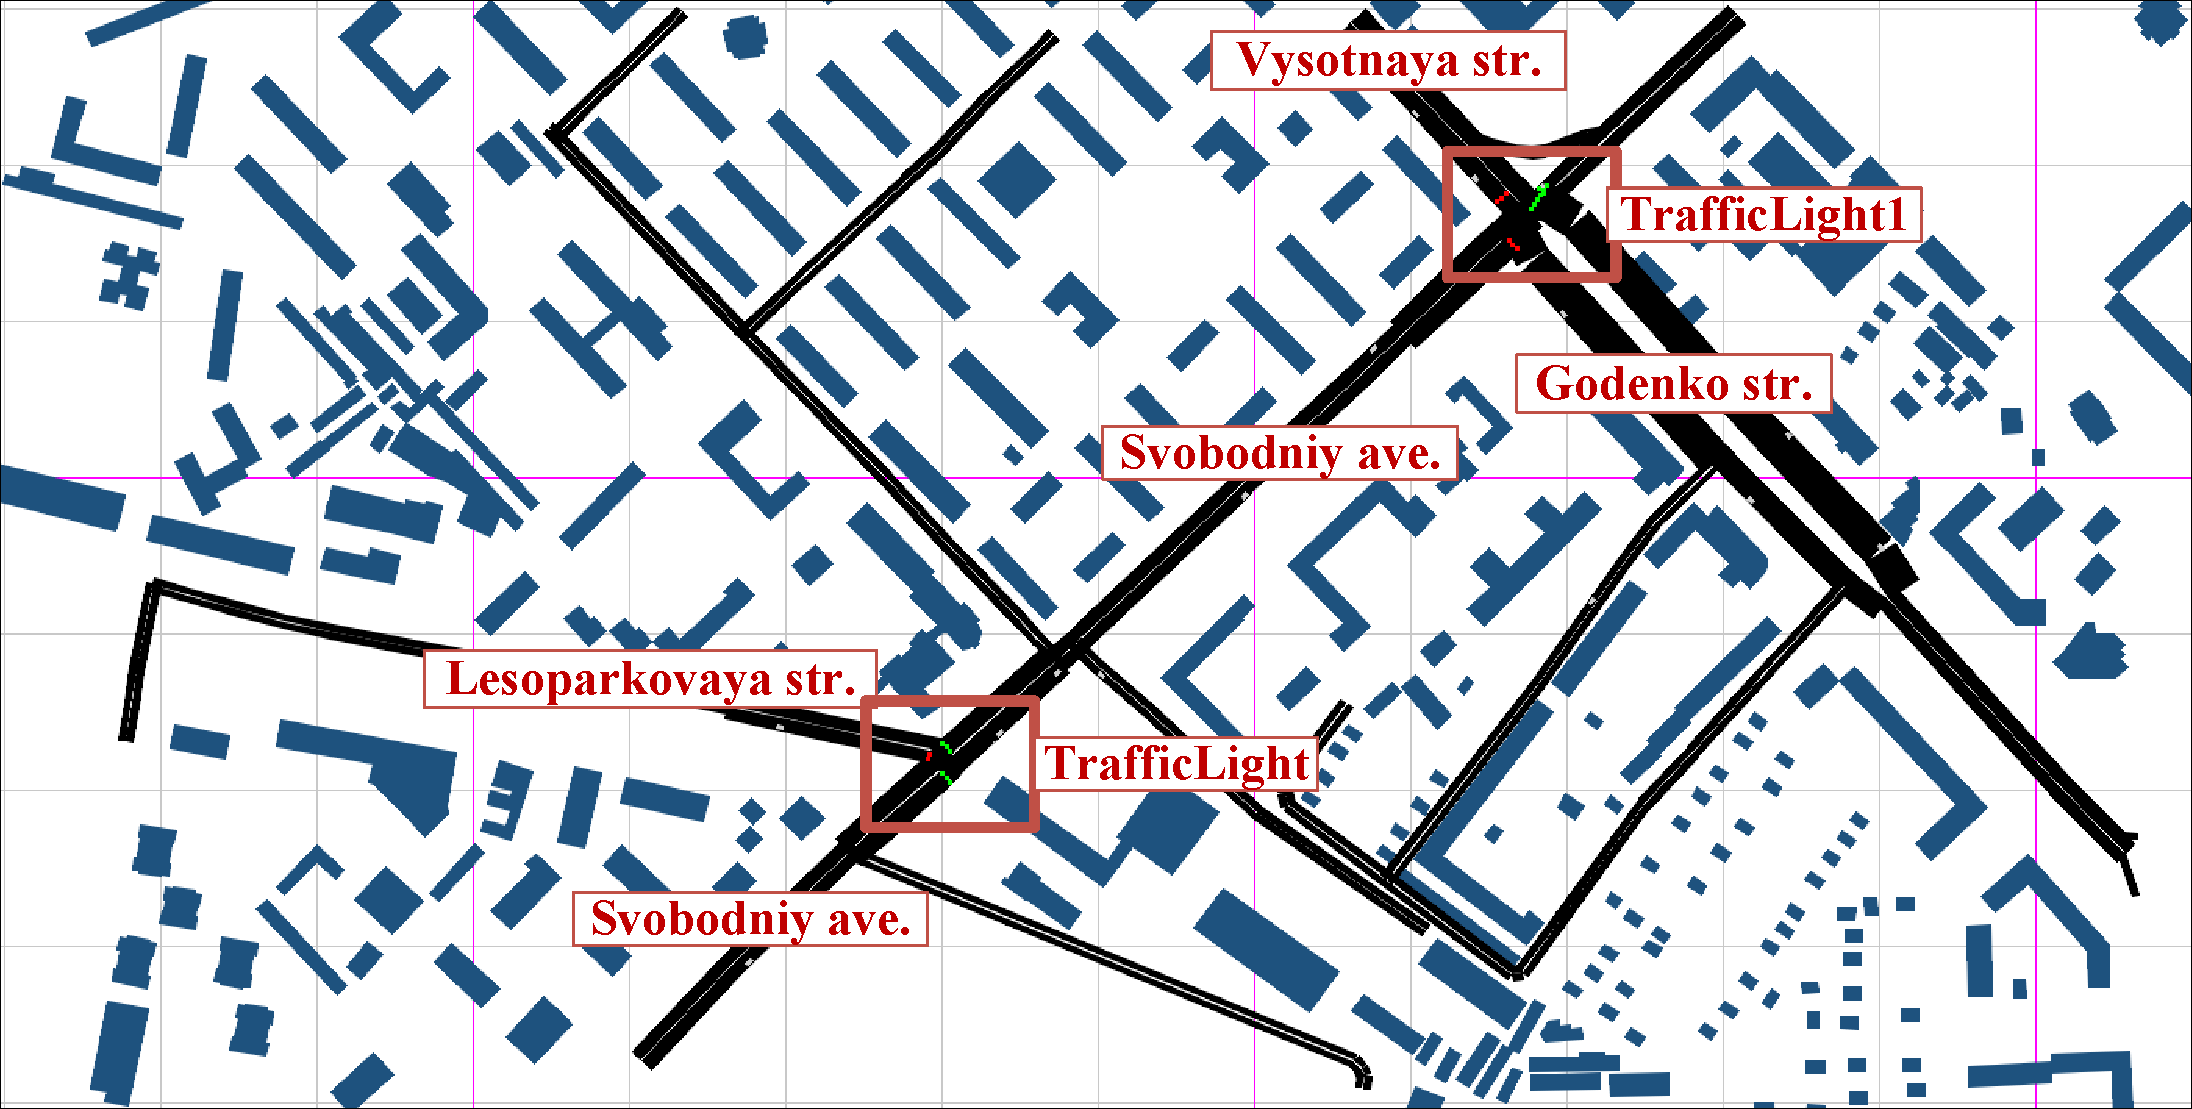
\includegraphics[width = 0.48\textwidth]{model_ex.pdf}
        �)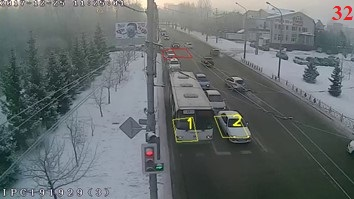
\includegraphics[width = 0.44\textwidth]{SV-LESOP_12.jpg}
    }
    \caption{�)�������� ���� ���������  MARLIN24; \linebreak �)���� ���������� �������� (����� ����) }
    \label{fig:ex3}
\end{figure}

���� ������������� ������� � ���������� ��������� ������������� ��������� ������� $X$ � $Y,$ ����������� ����� ������������� ������������ ������� �� ������� 1 � 2 �������������� �� ������ ������, ���������� � ���������� ���������� ������ ����������� � 2019 �� 2020 ���. 
�� ������ ���� �������� ������� ������ ��������� � ����� ������������ \cite{Epanechnikov}. ����� ������������� ���������� ������������� � ���, ��� ������ �� ��������������� ��������� ������� ����������� � ���� ����� ���������� �������������. 
� �������������� EM-��������� \cite{EM}, �� ���� �������� ����������� �������� ������� ������ ���������, ������������ ��������� ������.


��� ����� ������������� �������������  �������������� �������������� ���� ����������� ����������� ������ ���������� ������������ �����-����� ���  ���������  �������� ��������� �������� $(X,Y)$ \cite{Voitisheck, TOMSK}.
% \begin{description}[itemsep=-3pt]
%   \item [\sf{���� 1:}] ���������� ���������� �������������� �� ������� $[0;\;1]$ ��������� �������� ${l}, {w};$
%   \item [\sf{���� 2:}] ���� ����������� $\sum\limits_{m=1}^{M} p_m <{l}< \sum\limits_{m=1}^{M+1}p_m,$ �� ������� ������������� $M$-� ���������� �����  $F = F_M;$
%   \item [\sf{���� 3:}] ���������� ����� 2, ��� ${w}$ ���������� ������� ������������� ���������� ����� $G;$
%   \item [\sf{���� 4:}] ���������� ��������� �������� $(U,V)$ ��������~{\cite{nelsen2006introduction}};
%   \item [\sf{���� 5:}] ��������������� $U$-�������� $X_U$ ������������� $F;$
%   \item [\sf{���� 6:}] ��������������� $V$-�������� $Y_V$ ������������� $G.$
% \end{description}
����������  ����� �������������  �� 10-� �������� EM ��������� � ��� ������������ ����������  ������������� ��������� ������� $X$  � $Y$ ��������� �� �������~\ref{fig:margin}�) � ������� \ref{fig:margin}�).
\begin{figure}[tbph]
  \centering
  �)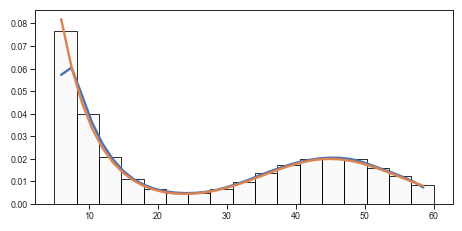
\includegraphics[width = 0.4\textwidth]{EM_yad_oc_dens1.png}
  �)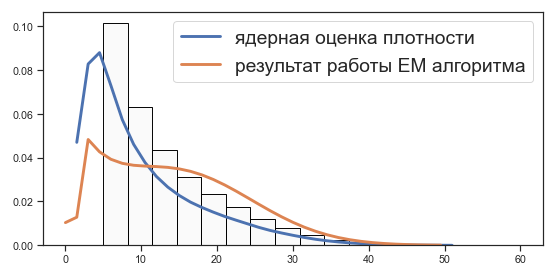
\includegraphics[width = 0.4\textwidth]{EM_yad_oc_dens2.png}
  \caption{���������� ����� �������������: ������ ���������� ������������ ����������: �) $X$; �) $Y$}\label{fig:margin}
\end{figure}

����������� �������, ���������� �������������� ������� ��������-������ � ����������� \(\alpha=0.9, \beta=0.25\) ������������ �� ������� \ref{fig:revive_distrib}.
\begin{figure}[tbph]
  \centering
  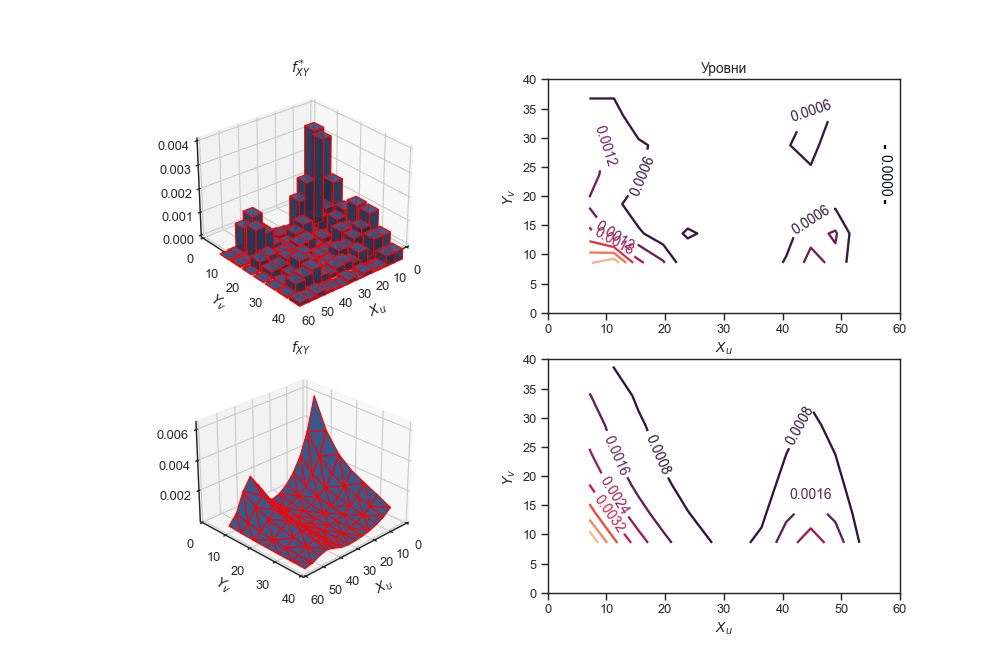
\includegraphics[width = 0.65\textwidth, trim={6cm 0cm 2cm 0cm}, clip]{EM_revive_density_function.png}
  \caption{��������� ������������  $F_{XY}^{*}$  � ������������� $F_{XY}$ ������� ������������� $(X,Y)$ ��� �������������   ������ ��������-������ � �����������  $\alpha=0.9, \beta=0.25$ }\label{fig:revive_distrib}
\end{figure}


\section{������ ����������� ���������� ������������ ���������}
\label{par:MARLIN2}

������ ������ ���������� ����������� ��������  ��� ������ ���������� ������� � �������������� �����.
����� (����������� ������) �� ����������� ��������� � ������ ������ ���������������� ��������� ��� ��� ���� ����. ��������� ��������� ���� �������� ������ �������� $\action$. \linebreak ����� --- ������������� ����������� �  ����������� ���������, ������� ���������� ������ �� �������� ����� �� ��� ������ �� ����-�����. ��������� ����� �������� ���������� ��� ����������� �������� � �����, ������� ������ ��������� � ������������� ����. ��������� ��������� ���� ��������� �������� $\state$.

� �������� �������������� ������ ���� ���������� � ������ ��������������� ����������� ���������� ������� � �������� ������ �������� �  ���������. %$\left\langle  \state, \action, \mathbb{P}, r \right\rangle$ .
����� �������, �������� ���������� ������������ ��������� �������� � ������ ��������������� �������� � ������������� (Multiagent Reinforcement Learning).





\subsection{������ ��������������� �������� � ������������� ��� ����������� ��������}
\label{subpar: MARL Q learning}
������ ��������� ����������� �������� (�������) � ������� ����������� �������� �������� ������� $\left\langle  \state, \action, \mathbb{P}, r \right\rangle$ \cite{SUTTON}.
������� �������� ������� ��� ������ ����� ��������� ��������� �������. � ������ ������� $t$ ����� ��������� ���������  ����� $s_t\in\state$ � �������� �������� $a_t \in\action$. ����� �������� ���������� ������ $R_t = r(s_t, a_t)$ � ��������� �  ���������
$s_{t+1}=s'$ \linebreak � ������������ $p(s' \bigm| s_t, a_t)$ �������� ������� ���������  $\mathbb{P}.$

  {
    ������� ������ ������������� ������������ ���������� $\delta= \{a_t, t \in \mathbb{N}\},$ ������������ ���������� ��������, \linebreak ${\cal T} = \left\{s_0,a_0, s_1,a_1, \dots, s_T,a_T \right\}$ ���������� ���  �������:
    \abovedisplayskip = -3.5em
    \begin{equation}\label{VALUE}
      \begin{split}
        V & = \sum_{t=0}^{\infty}\gamma^t r\left( s_{t+1} \bigm| s_t,\delta_t\right) 
        = \lim\limits_{T\to\infty}\mathbb{E}_{{\cal T}} \sum_{t=0}^{T}\gamma^t R_t,
      \end{split}
    \end{equation}
  }\noindent
���  ��������  $0 < \gamma < 1$, ���������� ������������� ���������� � ���������� �� ������� ��� ����������� ���������� �������������� �� ���� ��������� ���. 
���������� ������ ��������� ��������� ������� � ��������� ����� ����� ���������� ��� �� ������� ����� ��������� �����. 
�������������� ����� ������� $0 < \gamma < 1$ ������� � ���, 
����� ������������� �������������� ����������� $V.$

���������� ����������  ������ ���������� ������ ������������� ���������� ����������� �������� ������������ ����.
\begin{center}
  \begin{tabular}{rl}
    {\sf ����}:
     &
    \parbox[t]{0.84\textwidth}{���������� ������� �������� ������� $\left\langle  \state, \action, \mathbb{P}, r \right\rangle$ ���  ���������� ����������� ��������, ��������  � ��������� ������ ������� ���� ������������ ������� $s_0$.}
    \\
    {\sf  �����}:
     &
    \parbox[t]{0.84\textwidth}{
    ����������  ������������  ������� $\delta^*=\{ a^*_t\}_{0\leq t<\infty}$,\;\;\;\;  �������  �������� �������� ������� ������ ���\;\;\;\;\;\;\;\;  ������������� (\ref{VALUE}).
    }
  \end{tabular}
\end{center}

������� ������ ������  ������������ ����������� ���������� ������������ ��������� �������� ���� ������ ������� ������������� ���������������� �������� �������� ������������� ������---��������.
% \begin{proposition1}\label{prep:kropt}
� ������ ���������� ������ ������������ ������� ��������� ������---�������� ����� ��� \cite{My3}
  {
  \abovedisplayskip=0.5em
  \belowdisplayskip=0em
  \begin{equation}\label{BELMAN}
    V^* = \max_{a \in \action} \sum_{s'\in \state} p(s'\bigm|s, a)(r(s, a)+\gamma V^*(s')).
  \end{equation}}
  %��� ������������ ����������� �������� � �������� ������ �������� � ��������� � ���������  ������ (\ref{VALUE}).
% \end{proposition1}

������� (\ref{BELMAN}) ����� ���� ���������� � ������������ ������, ���������� $Q$-�������� \cite{SUTTON}.
������� ��������� �������������� ��� ����������� ���������� �� ���� $t$ ����� ���
{\abovedisplayskip=0.5em
\belowdisplayskip=0em
\[
  V^*\left(\{s_{t'}, \delta \}_{t'\in \mathbb{N},\;t'\leqslant t}\right)=\max\limits_{a\in{\cal \action}} Q_t(s_t, a).
\]}

�������, ��� ��� �������� ��������� ����� $s_{t+1}$ � ����������� ���������� $a_{t+1} $ �� ���� $t+1,$ ��������������� �������� ${l},$ � ���������, ��� �������� $Q$ ���� �� ������� $l$, �����
������� $Q$ ��� ������ ����������� � ����������� ���� 
\abovedisplayskip=0em
\belowdisplayskip=0.0em
\begin{equation*}
  \begin{split}
    Q_{l+1}(s,a) & = 
           \underbrace{p(s_{t+1}| s,a)\rule[-0.8em]{0em}{2em}}_{\alpha_{l}} \Bigl( r_{t+1} + \gamma V^*({s}_{t+1})\Bigr)  +                                                                         \\
                                     & + \underbrace{\sum\limits_{{s}' \in S/{s}_{t+1}} p({s}'| {s},{a}) }_{1-\alpha_{l}}\Bigl( r({s}'| {s},{a}) + \gamma V({s}') \Bigr) = \\
                                     & =\alpha_{l}\Bigl( r_{l} + \gamma\max\limits_{{s}'}Q_{l}({s}_{t+1},{s}')\Bigr)  + \Bigl(1- \alpha_{l}\Bigr) Q_{l}({s},{a}).
  \end{split}
\end{equation*}

���� ������  ������������ ����������� ���������� ������������ ��������� �������� ���� ����������� �  ���������� ������������� ����������� ��������������, ������������� �������� $Q.$ 
% \begin{proposition1}\label{prep:search}
   ��� ������ ������ ������������ ���������� ����������� �������� ����������� ��������� ����������� \cite{My3}:
  % \begin{equation}%\label{VALUE}
  %V(s) = \mathbb{E}\sum_{t=0}^{\infty}\gamma^t r(s_t,\delta(s_t)) \rightarrow\max\limits_\delta, s_0 = s
  % \end{equation}
  \begin{itemize}[itemsep=-3pt,topsep=0pt]
    \item ���������� ������������ ������ �������;
    \item ������ �������� �������������  ������� �� $n$-�� ���� ����� ���
          {
          $
            \rho(Q_n, Q_0) \leqslant \frac{\displaystyle \gamma ^n \rho(Q_1, Q_0)}{\displaystyle  1 - \gamma},
          $}\\
          \noindent
          ��� $Q_l \in \mathbb{R} _{\infty}^{| \action|+| \state|}$ --- ������� �������� $Q(s, a)$ �� ���� $l$,\\
          $\forall q,w \in \mathbb{R} _{\infty}^{| \action|+| \state|}$   ���������� 
          $\rho(q, w) = \max\limits_{ {\scriptstyle j\in \mathbb{N}, \rule{0em}{.9em}}\;{\mathmakebox[1em][l]{\scriptstyle j\leqslant {\left|\action\right|+\left|\state\right|}} }}\left| {q}_j - {w}_j\right|;$ % --- ������� ������������  $\mathbb{R} _{\infty}^{| \action|+| \state|}$, ������������ ��� $\forall q,w \in \mathbb{R} _{\infty}^{| \action|+| \state|};$
    \item ������������ ������� ��������� �������� ��������
          \begin{equation}\label{Voptsolve}
            V ^*(s) = \max_{a\in  \action}  \lim _{l \to + \infty}Q_l(s, a),     \end{equation}
          \begin{equation}\label{argoptsolve}
            a_t(s) = \arg  \max_{a' \in  \action} Q_l(s, a').  \end{equation}



          %$\left\langle {\mathbb{R} _{\infty}^{| \action|+| \state|},\rho(\cdot, \cdot)} \right\rangle$ --- ������ ����������� ������������ c 
          % $\forall q, w \in \mathbb{R} _{\infty}^{| \action|+| \state|}$ 
          %�������� $\rho(q, w) = \max\limits_{ 1\leqslant j \leqslant \left|A\right|+\left|S\right|} \left| {q}_j - {w}_j\right|,$ $\forall q, w \in \mathbb{R} _{\infty}^{| \action|+| \state|}.$


  \end{itemize}
  %������ �������� �������������  ������� �� $n$-�� ���� �������� ����� ���
  %  $$
  % \rho(Q_n(s, a),Q_0(s, a)) \leqslant \frac{\gamma ^n \rho(Q_1(s, a),Q_0(s, a))}{ 1 - \gamma}.
  % $$
% \end{proposition1}



\subsection{�������� ������}
\label{subpar: MARLIN24_descri}

�����  �������� ������� ������ ������������� ���������� ���������� ������������ ���������
������������ �� �������~\ref{fig:MARLIN_alg}.
\begin{figure}[tbph]
  \centering
  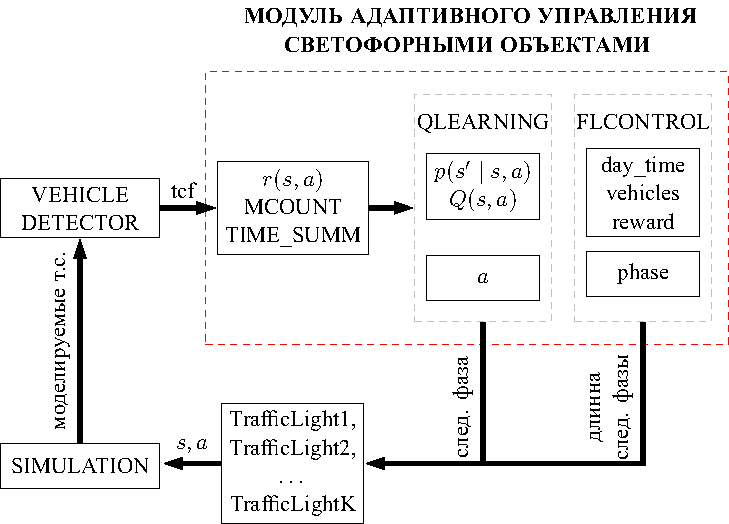
\includegraphics[width = 0.7\textwidth]{mod_scheme.pdf}
  \caption{����� ��������� MARLIN24 }\label{fig:MARLIN_alg}
\end{figure}
\textcolor{red}{}


� ������������ ����� (SIMULATION) ������������ ������������ ������ � ���������������, ����������� � ������ ���������, ���������� ������������ � ������������ ����� (SIMULATION) ����  �� ������ �� �� ���� ��������. 
��� ��������� ������ �� ������������� ������� �������� ���� $z,$ �� ��������������� ������,  ����������� ����������� ���������� � ���������� �������� (VEHICLE DETECTOR), ����, ��������� �� ���������� �� ������ ������ � �������� ������� ������, ����������� � ���� �� ��������� tcf (time collection forward) 
��� ���������� ������� ��������� ����������� �������� TrafficLight1, \dots, TrafficLightK. 
�� ��������� ���� ��������� ������ ��������� �� ��������� tcf, ��� ������� ����� ����. 
� ������� ������� ������� $dt$ �� ��������������� ������ ������ ���������� ���������� ������� ������������ ��� (QLEARNING),
% ����� ������ �� ��������??? \cite{Ivanov,Gasnikov} 
����������� ���������� �������� ��������� ��������� ����������� ����������. 

� �������� ������������ �������� ������������ ��� ���������  (QLEARNING), ��������������� �� ��������� �  ������ �����������  ���������� ������������ ���������, �����  ������� ��������� ������������ ���� � ��������� �����. ������ ������ ��� ������� ���������� � ������� ����������� �������� ������ (FLCONTROL) � ������ \cite{My3}. ��� ���������� ���������� �� ������ ������ ������� ����������� ������� ���� MISO (Multiple Input Single Output) � ����� ������� \cite{refarticle24}. 

��������� ��������������� ���������� ��������������� � �������� ������� ������:
����� ����� � ���������� ������ ${\cal{DT}} = \{\text{morning}, \text{day}, \text{evening}, \text{night}\},$
��������� �������� � ���������� ������ ${\cal V} =  \{ \text{run}, \text{wait}, \text{jam}\},$
����� ���������� � ���� �������� � ���������� ������ \linebreak ${\cal R} =  \{\text{small}, \text{medium}, \text{large}\}.$
��������������� ���������� ������ ����������� --- ������������ ����, ������������ ���������� ������  $P=$ 
\{ {long}, {medium}, {short}\}.  
���� ������ ������������ ����������� ��������� (�������~\ref{table:FL_rules}) ���������� ����:
\begin{equation*}
\begin{split}
    R:  &{\rm IF}\  (day\_time = A)\ {\rm AND}\  (vehicles = B)\  {\rm AND}\  (reward = C) \\
    &{\rm THEN}\  (phase = D),\;\rm{WHERE}\; A \in {\cal DT}, B \in {\cal V}, C \in {\cal R}, D \in {\cal P}.
\end{split}
\end{equation*}


\begin{table}[h]
  \caption{����� ������ ��������� ������}
  \label{table:FL_rules}
  \centering
  \scalebox{0.75}
  {
  \begin{tabular}{c|c|c|c|c|c|c|}
  \cline{2-7}
                                  & $R_1$ & $R_2$ & $R_3$ & $R_4$ & $R_5$ & $R_6$  \\ \hline
  \multicolumn{1}{|c|}{$day\_time$} & morning  & night  & -  & -  & day  & day  \\ \hline
  \multicolumn{1}{|c|}{$vehicles$}  & -  & -  & -  & run  & jam  & -   \\ \hline
  \multicolumn{1}{|c|}{$reward$}    & -  & -  & small  & -  &medium & medium  \\ \hline
  \multicolumn{1}{|c|}{$phase$}     & short  & short  & short  & short & short  & medium   \\ \hline
  \end{tabular}
  }

  \medskip
  
  \scalebox{0.75}
  {
  \begin{tabular}{c|c|c|c|c|c|c|}
  \cline{2-7}
                                 &$R_7$ & $R_8$ & $R_9$ & $R_{10}$ & $R_{11}$ & $R_{12}$ \\ \hline
  \multicolumn{1}{|c|}{$day\_time$} & evening &  day   & evening  & -   & -   & -   \\ \hline
  \multicolumn{1}{|c|}{$vehicles$}  &  -  & -  & -  & wait   & jam   & jam   \\ \hline
  \multicolumn{1}{|c|}{$reward$}    &  medium  & large  & large  & medium   & large   & small   \\ \hline
  \multicolumn{1}{|c|}{$phase$}     &  medium  & long  & long  & long   & long   & short   \\ \hline
  \end{tabular}
  }
  \end{table}

�� ������ �������� ������ ������ ����������� ������� � ������������ ���� ���������� ��� �� ��������� ������������ ��������� ����. % (��. ���. \ref{MARLIN_mod}).



\section{�������������� ������������}
��� ������������ �������������� � ������ ������� ���� ��������� ����� �������������� �������������. ������������ ����������� �� �� � ����������� Intel Core i7-10510U CPU@1.80��� � ����������� ������� ������� 8��.

������ ��������� ������� �������� �������� ���������� $\hat{\pi}(a| s),$ �������� �� ����������� ����� ��������� MARLIN24 �� ������� \ref{fig:structure_MARLIN24}.
������ ����������� ���������� ������������ ��������� ��������� ����������� ���������������� ���� trafficLightConfig.xml. � ���������������� ����� ���������� ���������� � ��������� ������������ ��������, ���������� ��� � ������ ����������� ��������.
�����  �������� ����������� ������� MARLIN24  ���������  ���������  ������� � ������������ ������  � ������������ ����������� ���������� ��� ����������� ��������.

���������� ������� (VEHICLE DETECTOR) � ������������ ����� (SIMULATION)  ���������� ������ ��������� $t_i$ ���������������� ������������� �������� $i \in I \subset \mathbb{N}$ �  ���� $z\in Zones  = \left\{z^{(0)}, z^{(1)}, \dots, z^{(m)} \right\}, m \in \mathbb{N}$.
�������, ��� ��� ������������ �������������   ��������������� ������������� �������� ������������ ������� ����� ������ ��������������. ��� ��������, ��� �� ����� ��������������� ��������� ��� $(i,z),$ ���  ���������� $i$ ��������� � ������������� ���� $z$ � ������ ������� $t.$ ��������� ������ ��������� ��� ��������� $\psi_t \subset \mathbb{N} \times Zones, $ ��� ��������  $i\psi_t z.$
������ ����� ��������� $\phi \subset Zones \times \state,$ ����������� ���� $z, $ � ������� ��������� $s'$ ��������� ��������.
����������� ���������� �  ����� � ������������ � ����� ������������ ������� $s'$, ������� ��������� �������� ������������ ������� � ���� ����� � ���������
$
  I(s',t) = \left\{i|\;\; t_i < t, i \psi_t z, z \phi s' \right\}.
$

�������� �����������, ������ �� ������� ��������� ������� ��������������.
��� ������ ������ ���������� ����� �����  �� ������� ������, ������������ � ��������� � ��������������� ����-������ �����������.
�����  $r:  \state \times \action \mapsto \mathbb{R}$ --- ������� �������������� ������ ��� ��������� ������������ ��������� $s_t$ ��� �������� $a_t=\delta(s)$. 
� ������ ������� $t$ �������� ������� $r(s_t, a_t)=R_t$  ������������ ��� ��������� �������� ������ � ��������������� �������, ������������ ����� �������� �� ����������� ������������� �������� ������ $R_t = \sum\limits_{\mathmakebox[1em][l]{i \in I(s',t)}} (t -t_i).$

����� ��� ������������ ��������� ����������� �������� $TL$  � ��� �������� $z$ ������������ ������� ������ $r(s,a)$ ����� ���������� ����� (MCOUNT), ��������� ����� ������� ����� ������������� ������� �������� ���� (TIME\_SUMM) �  ��������� ������� $Q.$
��� ���������, �����������
��������� �������  ${\cal X}=\left\{(s_i, a_i)\right\}_{i=1}^T$
������� $T$ ������� $10^6$. � ����������  ���������� $\delta^*,$ ��������� �� ����������� ���������� �������� ������� ������ ������������� $Q,$  ��������������  ����������� ������
������������� ${\cal P}=\{p(s, a)|\; s\in{\state}, a\in{\action}\}$ ��������� ��������� �������� $(s, a)$, ��� ������� 
$p(s, a)$  --- ����������� ����, ��� � ��������� $s$ ����� ������ ������� $a$.
�� ���������
���������� ������������  $\hat{p}(s, a)$ ����������� ������
�������� ������ $\hat{\pi}(a| s)$  ��� ������� $s\in\state$
$$
  \hat{\pi}(a| s)=\frac{\hat{p}(s, a)}{\displaystyle \sum\limits_{a\in{\mathbb A}}\hat{p}(s,a)}=\frac{\hat{p}(s, a)}{\hat{p}(s)}.
$$
%�� �������� ��� ������� ������ ������ ������������� $\perprob\left(s , a\right)$ ����������, �� �.�. ����������� ������� ������� ������� $10^6$, �� �� ��� �������� ������������ ������� ������������� ��������� ��������. �������� ������ ������� �����
% (������ �� ���������� ����������  
%��� ��������� � ������� ���������  ������������ ������� ������������� $\perprob^*_n\left(s , a\right).$
% ������ � ���������� ������, ��� ��������� �������������� ������������ �������  $r_{a^{(k)}} =\left\{r(s_0,a^{(k)}),r(s_1,a^{(k)}),r(s_2,a^{(k)}),\dots\right\}$, $ k\in K$.
% �������� �������� $r\left(s_t,a^{(k)}\right)$  --- ����� ���������� ����� �� ������������  ������� $k$ � �����  $a^{(k)}\oplus s_t$  �������. %������ ������� ���������� � ������� ����������� ������ ���������.
% ��������� ��������� ������������� ������� ����������� �� ������� \ref{fig:intens1}.
% \red{�������� �������}
% \begin{figure}[H]
%     \centering
%     %\includegraphics[width=0.99\textwidth]{exintens.png}
%     \caption{������������� ������� �� ����������� � ������� 24 �����, ������� ���� ������������� ���� $s^{(0)}$, ������� --- $s^{(1)}$}
%     \label{fig:intens1}
% \end{figure}
\label{par:computation}

� ���� ����� �� 1000 ��������� ���� ��������� ����������� ������ ��������  ������� ������ ������������� ���������� $\hat{Q}$  ��� ����������� �� ���� ��������� \cite{Nash}.
������ �������� ��������� �� �������~\ref{fig:strategies}, ��� ����� ������ �������� ������� ����������� �������� $Q$ ��� ������ �����  �� ���������� ������� $t$, ������� ������ --- �� ����������� �������� $\hat{Q}.$
\begin{figure}[tbph]
  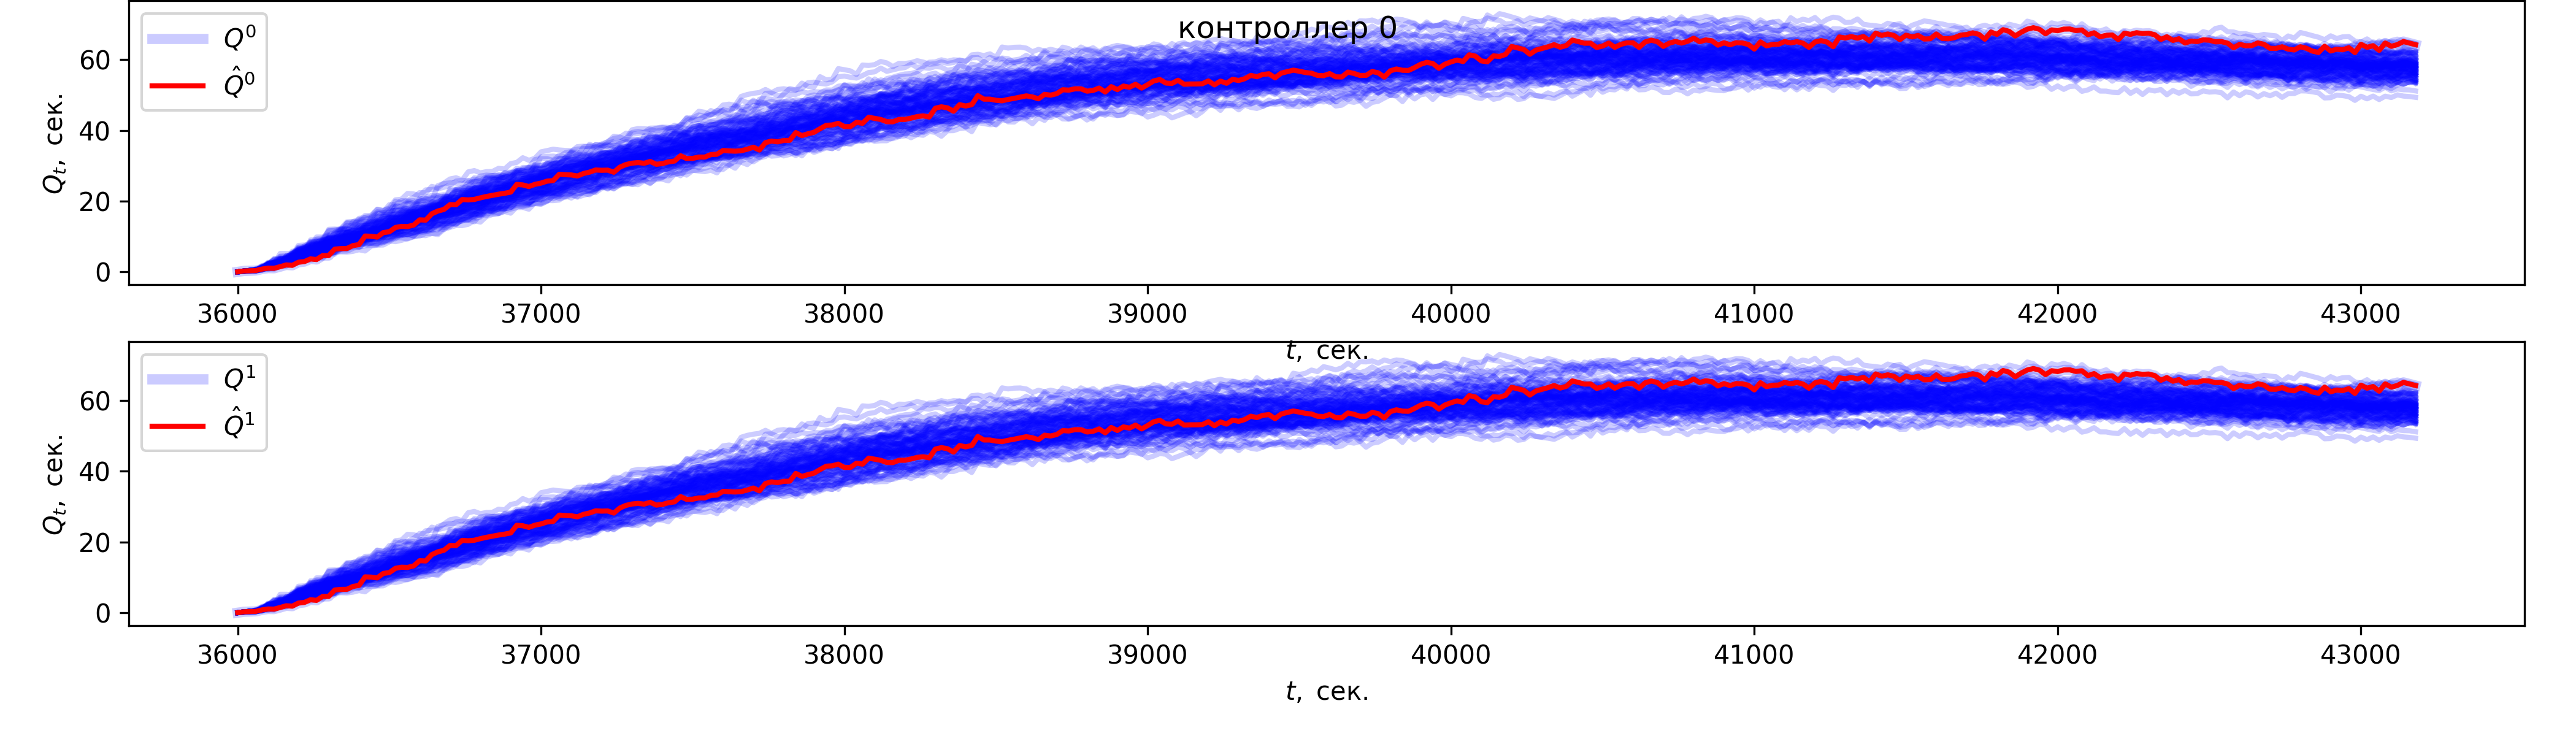
\includegraphics[width=0.99\textwidth]{learningcurve40.png}
  \caption{������ ���������� ������ �������� $Q$  }\label{fig:strategies}
\end{figure}


% ���������� �������������� ������������� �������������
%  ������� ������ �������� $Q^i$ ��� ����������� �������� $0,1$ ��� ������� ������������� ������ ������������ ��������� $\mathcal{O}$ � ��� �������, ����� ��� ��������� � ������ ������������� ��������� $\mathbf{\state};$
%  ���������� ������������� ���������� ��� �����24 � MARLIN24.

% \begin{table}[tbph]\footnotesize
%   \caption{������� ������ ��������}\label{table:strategies}
%   \centering
%   \begin{tabular}{|p{0.1\textwidth}|l|}\hline
%     \rotatebox[origin = c]{90}{\parbox[s]{0.25\textwidth}{\centering ��������� �����\\$\mathcal{O}\subset \state^0\times\state^1,$                                                                                                                                                   \\ $\mathbf{\state} =  \state^0\times\state^1\times\state^2$}}	& \parbox[s]{0.85\textwidth}{\centering 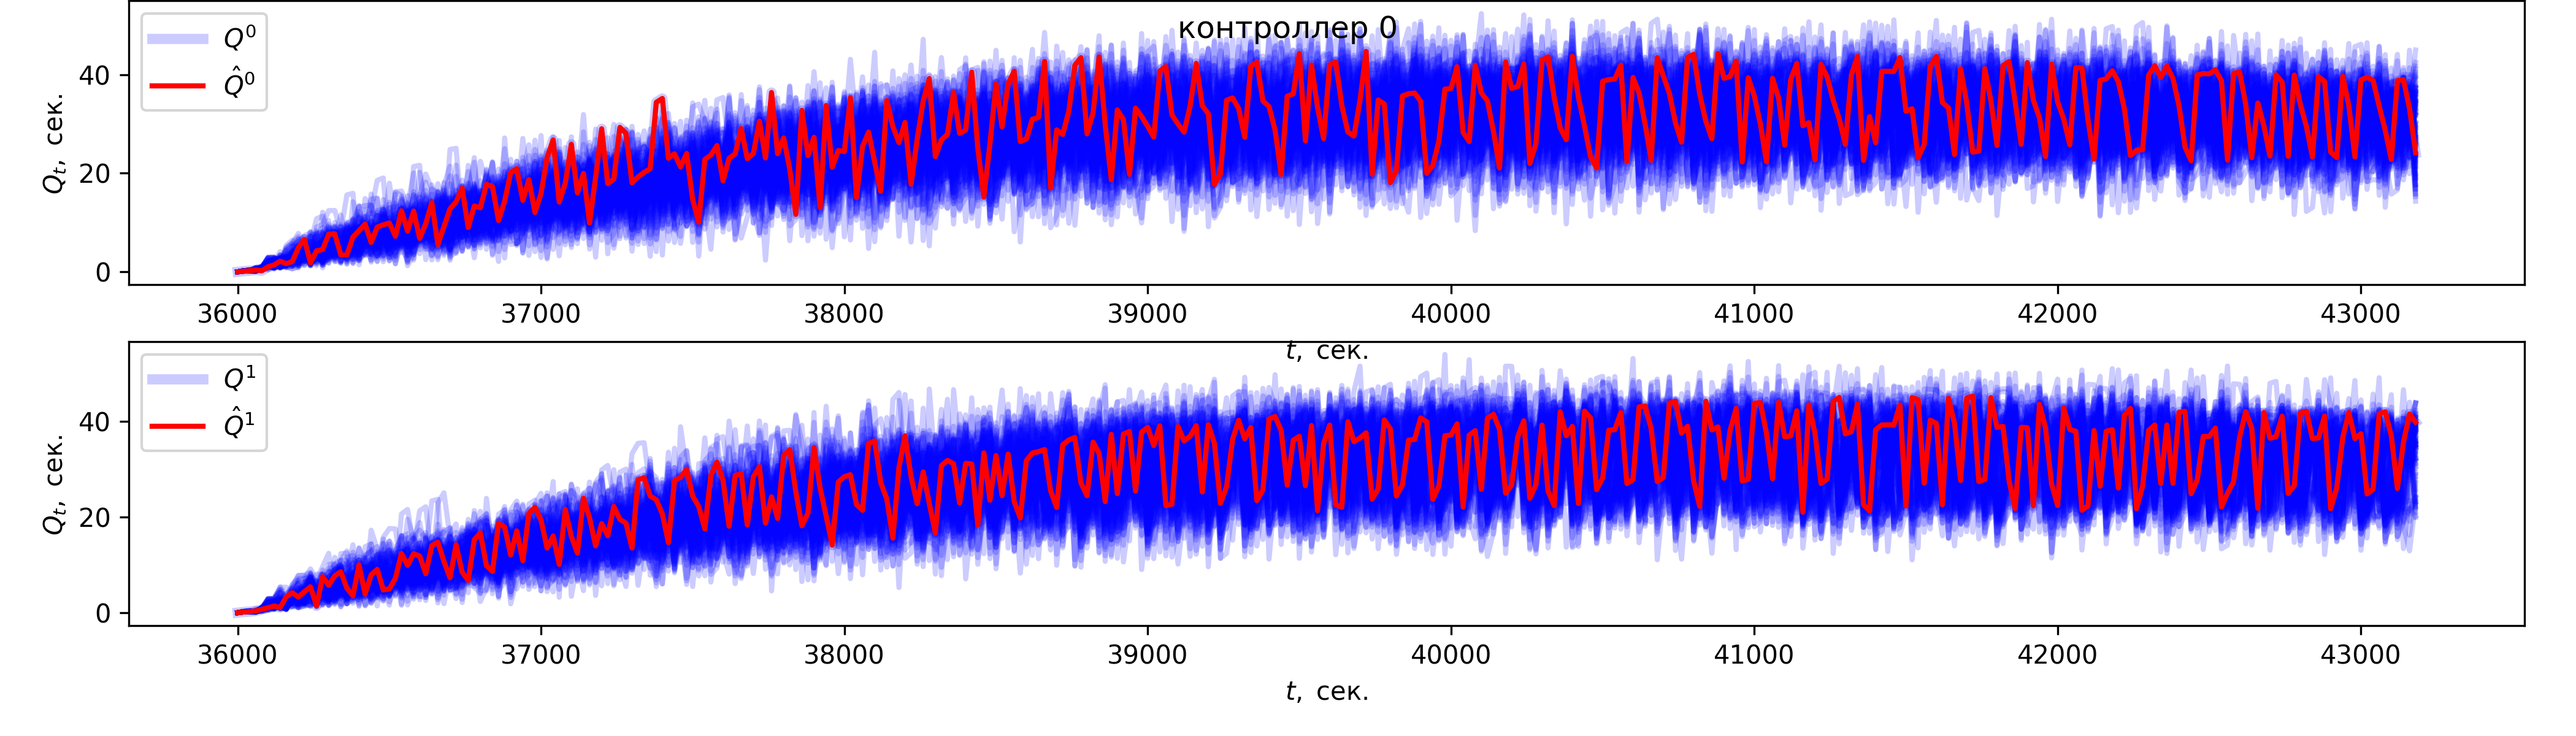
\includegraphics[width = 0.85\textwidth]{learningcurve20.png}\\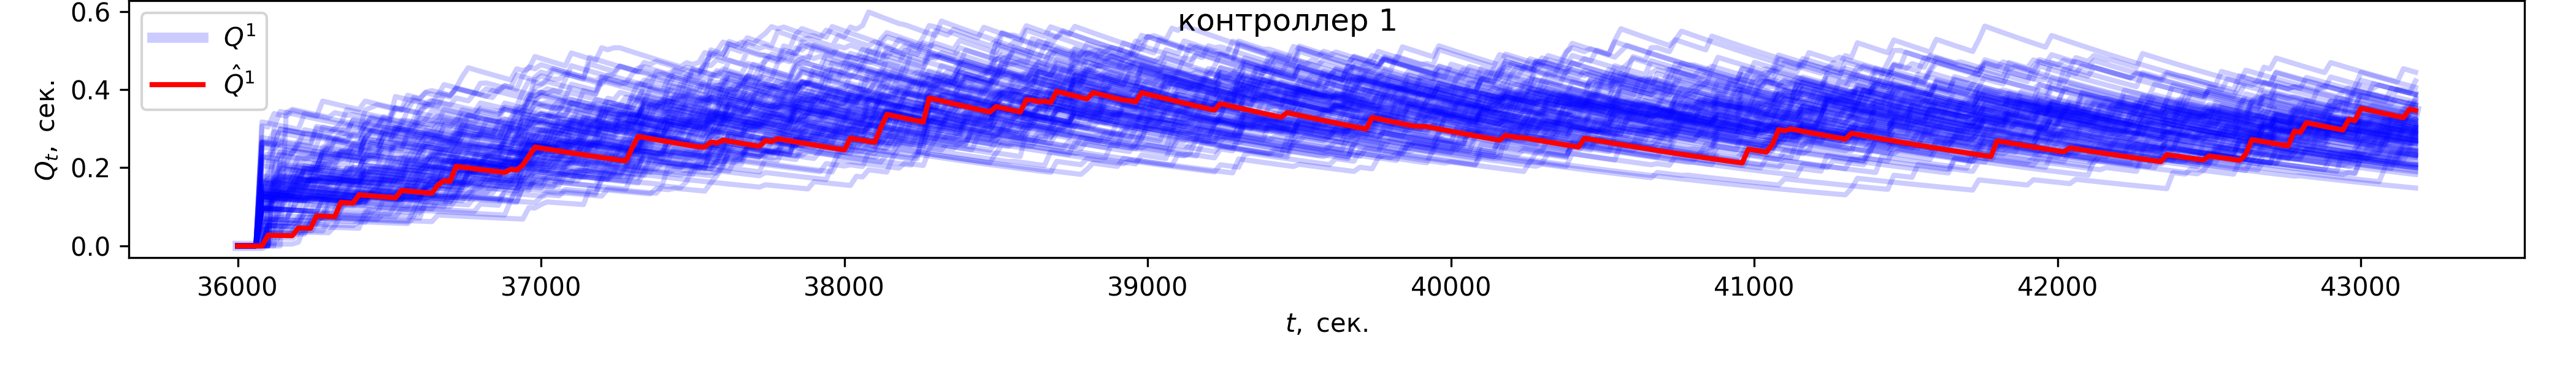
\includegraphics[width = 0.85\textwidth]{learningcurve21.png}  }\\\hline
%     \rotatebox[origin = c]{90}{\parbox[s]{0.3\textwidth}{\centering  ������ �����\\ \; \\ $\mathcal{O} =  \mathbf{\state} = \state^0\times\state^1\times\state^2$}} & \parbox[s]{0.85\textwidth}{\centering 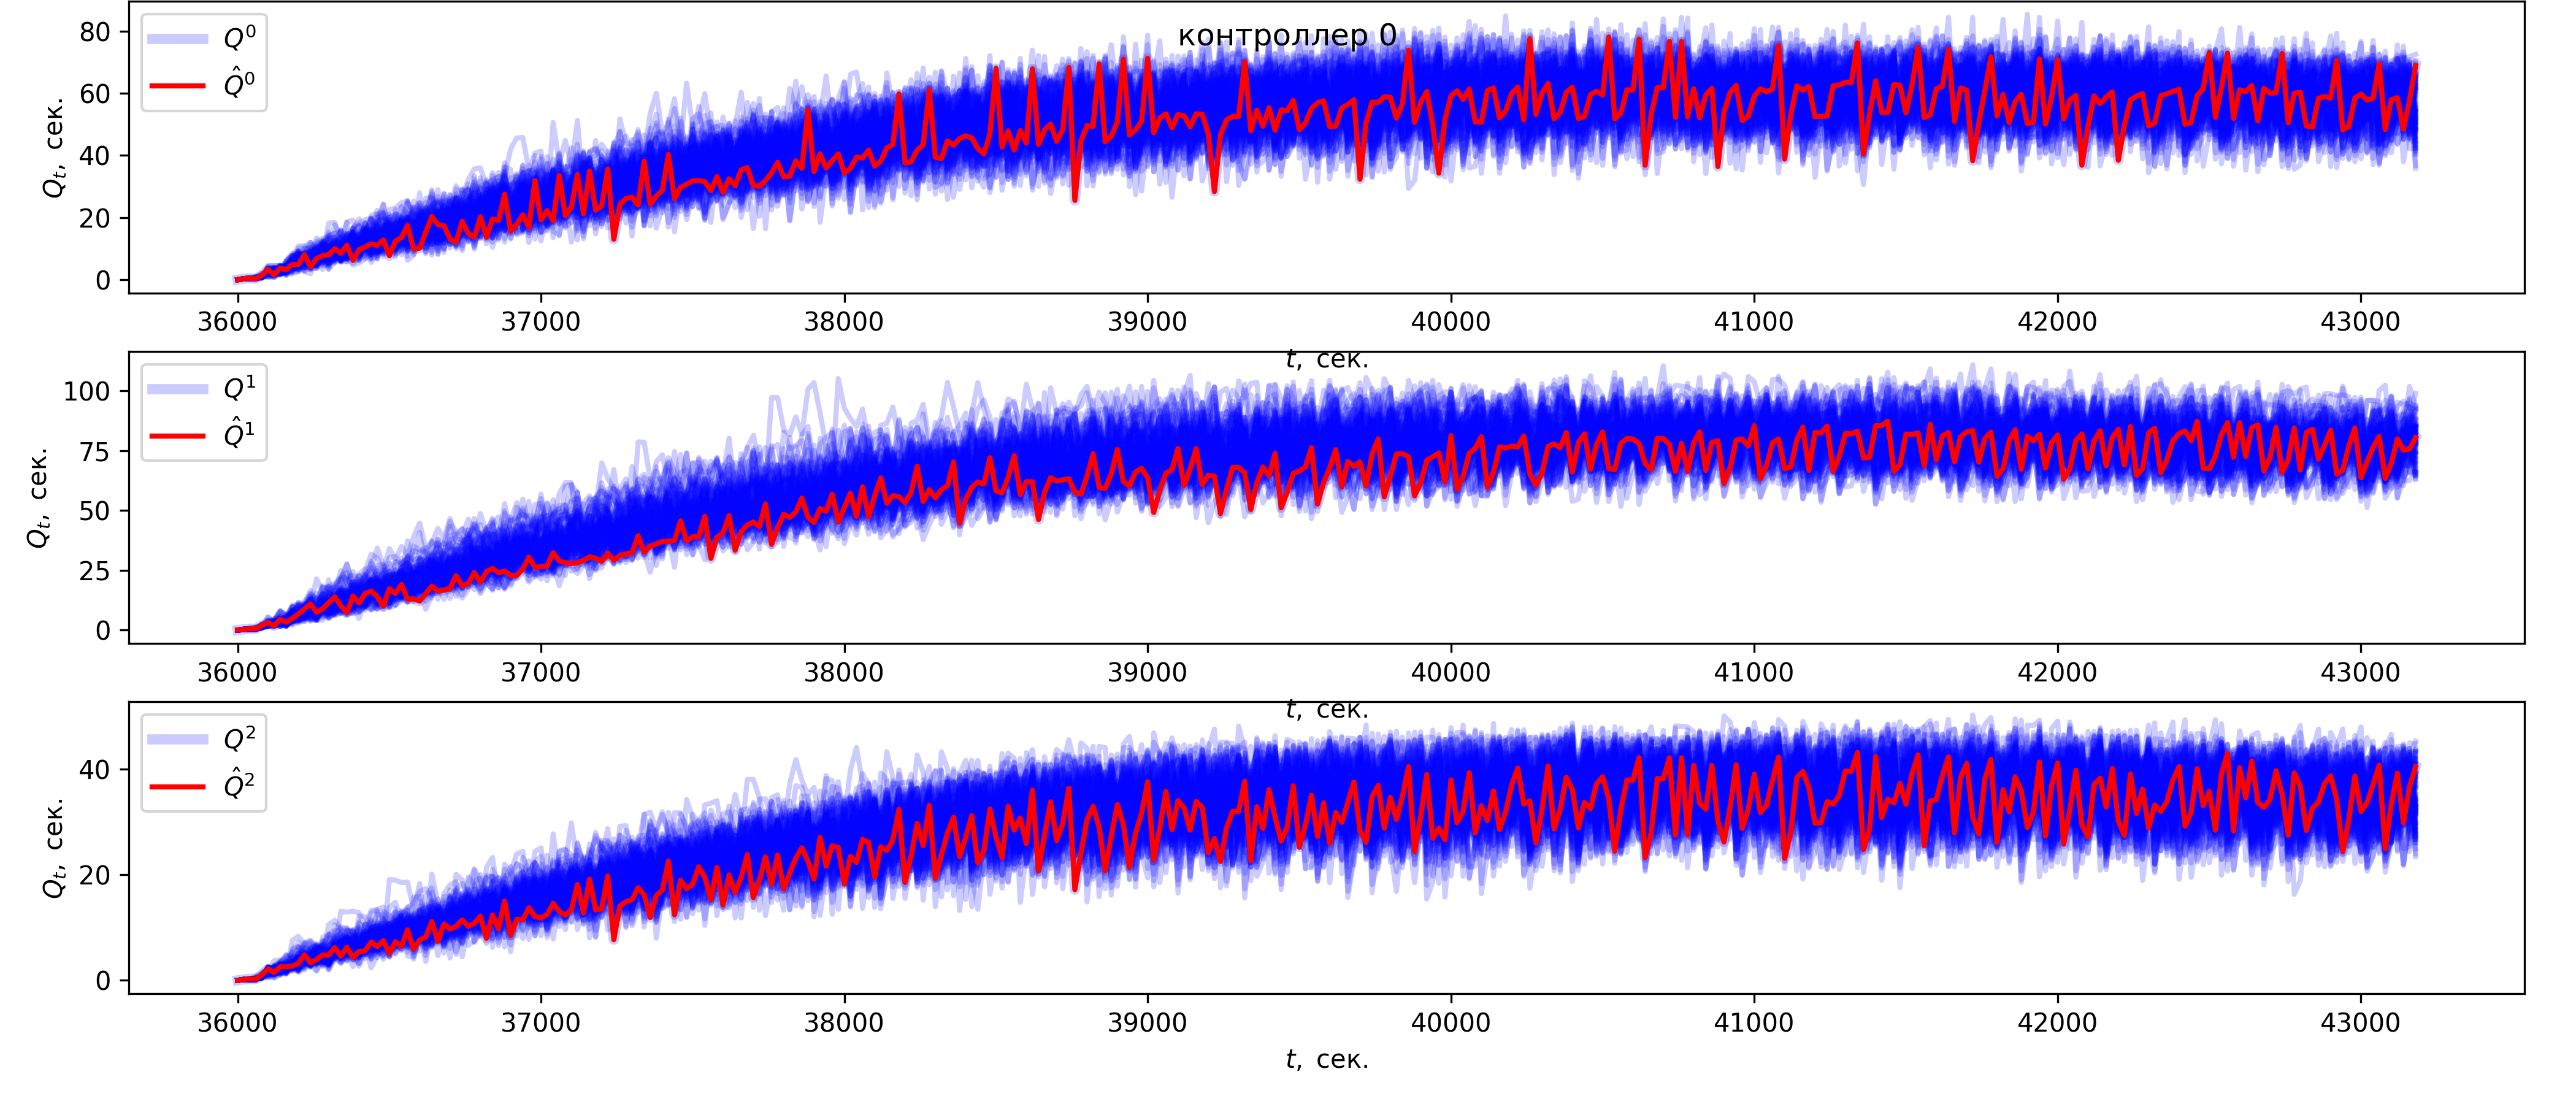
\includegraphics[width = 0.85\textwidth]{learningcurve2.png} } \\\hline
%   \end{tabular}
% \end{table}


% �������, ��� ��� ������������ ������� ������������ ���������, ��������� ����� ���������� ������������ �� �������, ������������� ������� ������������ �������, ����������� ������, ��� �� $0$ � $1$-��,  � ������� � ������ ������� ������ ��� �� ������� ������ � ���������  ����������. 

� ������ �������������� ������������� ���� ��������� ��������� ������ ��������  ������� �� ���������� 1000 ����. 
� ���������� ������������ ���������� ����� �������� ������������� �������� � ������� �� ��������� ����� ����� ������������ �������. 
����� ���� ������������������, ��� ������������� ��������� ���������� ��� ���������� �������� �������� ���� ����� � �� ����. 
����� �������, ���������������� ���������� ������������ ��������� � ����� ��������� ���������� ����� ���� ����������� ������ � ��� ��������, ��� ��� ���������� ���� �������� ��������� � ����������. 
� ��������� ������� ����� ���� ���������� ������������������ ������, �, �������������, <<��������� �����������>>, ����������� � ������ ����������� ������ ��� �����������, �� �������� ��������� ���������.

� ������ \cite{My2} ���� ��������� ��������� ����������� ������������� ����������  � ��������� MARLIN24 � �����24.
�� ����������� ������������ \cite{My2}, ���� �������� ������������ ���������� ��� �������� ������� �������� �� ��������� �������� ��� ������, ����������� ���������� ��������� �������� ������� MARLIN. ������ ��������� ������������� ��������� ���������� ���������� ������� ����������� �������� ����� ���� ��������� ��� ��������� ������� �������� �������� ����.

����� � ������ \cite{My3}  ���� ��������� ��������� ����������� ������������� ����������, ������������ ��� ����������������� ����������� ���������� ������������ ���������  ������� �������� ���� (MARLIN), ������������������� ����������� ���������� (MARL), ��� ����������� �������� � ������������� ��������������� ������ (FIXED) � � ���������� ������������� ��� (FUZZY) �� ����������� ������������, ���� �������� ������������ �������  ��� �� $30\%$ ��� �������� ������� �������� �� ��������� �������� ��� ������, ����������� ���������� ��������� �������� ������� MARLIN.

\section{����������}
� ������ ������� ������������� ���������� ���������� ������ ��������� ������������ ��������� MARLIN24 ��� ����������� ���������� ������������ ���������. ���������� ����� ��������� �������� ��������� �����������. ��-������, ��������� ������� ������������� ��������� �������, ����������� ������������� �������� ������������ ������� �� �������. ��-������, ��������� ����� ������� ������������ ��������. �-�������, �������������� ������� ����������� ������������ ��������� �������.

������ ���������� ������������ ������������� ������������� ����� ��� ������������� ������������ �������, �������� � �������� ������������ ������������ ����������. � ���������� ����������� ���������� �������������� ������������ ��� ������ �������� � ������������ ���������� ������� � �������� �������� �������� ����, � ����� �� ���������� � ������� �������� ��������� MARLIN24.
% \begin{table}[tbph]
%   \centering
%   \caption{��������� ����������� ������������� ���������� ��� ��������� �������}
%   \label{table:compar1}
%   \scalebox{0.8}{
%     \begin{tabular}{|c|c|>{\columncolor{blue!20}}c |>{\columncolor{red!20}}c |  c|}
%       \hline
%       \parbox[s]{6em}{\rule{0em}{1.2em}������� �������}                                                   &
%       \parbox[t]{2em}{��.                                                                                   \\ ���.} &
%       \parbox[s]{5em}{\rule{0em}{1.2em}�����24}                                                           &
%       \parbox[s]{5em}{\rule{0em}{1.2em}MARLIN24}                                                          &
%       \rotatebox[origin=B]{90}{\rule{0.2em}{0em}���������\rule{0.2em}{0em}}
%       \\
%       \hline
%       \mbox{\parbox[s][1.2\height]{6em}{\rule{0em}{1.5em}�������                                            \\ ��������}}&
%       $\frac{\rule[0.2em]{0em}{1.5em}\displaystyle\text{c��.}}{\rule{0em}{1em}\displaystyle\text{���.}} $ &
%       10.63                                                                                               &
%       9.4                                                                                                 &
%       11.6\%
%       \\
%       \hline
%       \mbox{\parbox[s]{6em}{\rule{0em}{1.5em}����������                                                     \\ �����������\rule[-1em]{0em}{1em}}}&
%       ���.                                                                                                &
%       4 870                                                                                               &
%       4 412                                                                                               &
%       -9.4\%
%       \\
%       \hline
%       \mbox{\parbox[s][1.2\height]{6em}{\rule{0em}{1.5em}���������                                          \\ �����}}&
%       ���.                                                                                                &
%       51 792                                                                                              &
%       41 286                                                                                              &
%       20.3\%
%       \\
%       \hline
%     \end{tabular}}
% \end{table}
\noindent


% \section{Описание задачи для одного агента}
% \label{par:MARL_description}


% Как правило, обучение с подкреплением используется для одного агента в среде, чтобы максимизировать его долгосрочную награду. В работе исследуется модель обучения с подкреплением нескольких агентов (светофорных объектов) в стохастической среде. Обучение с подкреплением сводится к оптимальному сопоставлению агентом действия $a$ состоянию среды $s$. Предложенная математическая модель процесса выбора фазы светофора учитывает текущее расположение светофоров и их загрузку и позволяет сформулировать оптимизационные задачи, целью которых является минимизация задержки движения автомобилей. Отметим, что структура мультиагентной системы обеспечивает наиболее эффективное распараллеливание всей задачи на подзадачи.

% Введём следующие обозначения: $ \state$ --- дискретное пространство состояний, $ \action$ --- дискретное пространство действий агента, $\delta \colon \state\to \action$ --- 


\newpage
% Авторы - по алфавиту, сначала русскоязычные, затем остальные.
\begin{thebibliography}{10}
  \bibitem{transp_strat} Транспортная стратегия Российской Федерации, утверждена распоряжением Правительства Российской Федерации от 22 ноября 2008 года №1734-р. [Электронный ресурс]. – Режим доступа: {http://mintrans.gov.ru} (дата обращения: 25.06.2024).

  \bibitem{goel2017} S. Goel, S. Bush, C. Gershenson, "Self-Organization in Traffic Lights: Evolution of Signal Control with Advances in Sensors and Communications," University at Albany,  2017, pp. 1708.

  \bibitem{carini1977} R. N. Carini, {Application of the UTCS-1 Network Simulation Model to Select Optimal Signal Timings in a Multi-Linear Street System: Interim Report}, Publication FHWA/IN/JHRP-77/19, Joint Highway Research Project, Indiana Department of Transportation and Purdue University, West Lafayette, 1977.

  \bibitem{chandler1985} M. J. H. Chandler, D. J. Cook, "Traffic Control Studies in London: SCOOT and Bus Detection," OTRC Proc. Annual Summer Meeting, University of Sussex,  pp.111-128, 1985.

  \bibitem{gartner1990} N. H. Gartner, "OPAC: Strategy for Demand-responsive Decentralized Traffic Signal Control," IFAC Proceedings Volumes, vol. 23, no. 2, pp. 241–244, 1990. 

  \bibitem{asudd} ASUDD "Micro-M".

  \bibitem{IDM} M. Treiber, A. Hennecke, and D. Helbing, "Congested traffic states in empirical observations and microscopic simulations," {Transportation Physics Reviews E}, vol. 62, pp. 1805–1824, 2000.

  \bibitem{MOBIL} M. Treiber and D. Helbing, "Realistische Mikrosimulation von Stra?enverkehr mit einem einfachen Modell," in {16. Symposium "Simulationstechnik ASIM 2002" Rostock}, 2002, pp. 514–520.

  \bibitem{networkx} NetworkX Developers, {NetworkX}. [Электронный ресурс]. – 2024. – Режим доступа: {https://networkx.org/} (дата обращения: 25.06.2024).

  \bibitem{osmnx} Boeing, G., {OSMnx: Python for Street Networks}. [Электронный ресурс]. – 2024. – Режим доступа: {https://osmnx.readthedocs.io/} (дата обращения: 25.06.2024).


  
  \bibitem{nelsen2006introduction} Нельсен, Р. Б.,{An Introduction to Copulas}. Springer, 2006.--270с.

  \bibitem{marshall1996copulas} Маршалл, А., "Copulas, Marginals, and Joint Distributions," {Lecture Notes-Monograph Series. Distributions with Fixed Marginals and Related Topics}, 1996, no. 28, pp. 213–222.

  \bibitem{Quesada} Кесада-Молина, Х. Х., и Родригес-Лаллена, Х. А., "Bivariate copulas with quadratic sections," {Journal of Nonparametric Statistics}, 1995, pp. 323–337.

  \bibitem{Epanechnikov} Эпанечников, В. А., "Non-Parametric Estimation of a Multivariate Probability Density," {Theory of Probability and Its Applications}, 1969, pp. 153–158.

  \bibitem{EM} Бишоп, К. М., {Pattern Recognition and Machine Learning}. Springer, 2007.

  \bibitem{Voitisheck} Войтишек, А. В., {Основы метода Монте-Карло: Учебное пособие}, ред. В. Н. Задорожный. Новосибирск: НГУ, 2010. "--- 108 с.



  % \bibitem{shoufeng2008} L. Shoufeng, L. Ximin, and D. Shiqiang, "Q-Learning for adaptive traffic signal control based on delay minimization strategy," in {Proc. IEEE Int. Conf. Netw. Sens. Control}, 2008, pp. 687–691.

  \bibitem{el-tantawy2013} S. El-Tantawy, B. Abdulhai, H. Abdelgawad, "Multiagent Reinforcement Learning for Integrated Network of Adaptive Traffic Signal Controllers (MARLIN-ATSC): Methodology and Large-Scale Application on Downtown Toronto," {IEEE Transactions on Intelligent Transportation Systems}, vol. 14, no. 3, pp. 1140-1150, 2013.

  % \bibitem{el-tantawy2010} S. El-Tantawy, B. Abdulhai, "Towards multi-agent reinforcement learning for integrated network of optimal traffic controllers (MARLIN-OTC)," {Transportation Letters: The International Journal of Transportation Research}, vol. 2, pp. 89–110, 2010.

  \bibitem{sutton2015} R. S. Sutton, A. G. Barto, {Reinforcement Learning: An Introduction}, 2nd ed., The MIT Press, Cambridge, Massachusetts, 2015, pp. 145–147.

  \bibitem{tislenko2021} Т. И. Тисленко, "Задача MARL для светофора на перекрёстке",  Материалы VIII Международной молодежной научной конференции "Математическое и программное обеспечение информационных, технических и экономических систем", 2021, С. 144-149.

  \bibitem{tislenko2022a} Т. И. Тисленко, Д. В. Семенова, "Задача MARL для светофорной сети," in {Информационные технологии и математическое моделирование (ИТММ-2021): Материалы XX Международной конференции имени А.Ф. Терпугова}, Томск, 2022.

  \bibitem{tislenko2022b} Т. И. Тисленко, Д. В. Семенова, Н. А. Сергеева, "Оптимизация планов координаций для светофорных объектов участка дорожной сети," in {Системы управления, информационные технологии и математическое моделирование: материалы IV Всероссийской научно-практической конференции с международным участием}, Омск, 2022, С. 255-261.




\end{thebibliography}

\newpage
\makeenginfo
\makeauxinfo

\end{document}
